% =============================================================================
%  Major Technical Project - Final Report (IIT Mandi format)
%  Extreme Value-Guided Deep Generative Models for Imbalanced Classification
%
%  HOW TO COMPILE (Overleaf or any LaTeX compiler, pdfLaTeX):
%    Upload the whole zip as a new Overleaf project (New Project > Upload Project).
%    main.tex must sit next to the folder figures/, which holds every .png and diagram*.pdf.
%    The diagrams are ready-made PDFs (no TikZ), so the report compiles quickly.
%
% =============================================================================
\documentclass[12pt,a4paper]{report}

% ----------------------------------------------------------------- your details
\newcommand{\ReportTitle}{Extreme Value-Guided Deep Generative Models for Imbalanced Classification}
\newcommand{\ReportSubtitle}{Case study: Next-day extreme heat prediction in Himachal Pradesh}
\newcommand{\StudentName}{Divyansh Jain}
\newcommand{\RollNo}{B23397}
\newcommand{\SupervisorName}{Dr. Rishikesh Yadav}
\newcommand{\SupervisorTitle}{Mentor}
\newcommand{\SchoolName}{School of Mathematical and Statistical Sciences}
\newcommand{\ReportKind}{Final Report}
\newcommand{\ReportMonth}{November 2026}
\newcommand{\CertificateDate}{November 2026}

% ----------------------------------------------------------------- packages
\usepackage[a4paper,left=1in,right=1in,top=1in,bottom=1in]{geometry}
\usepackage[T1]{fontenc}
\usepackage{amsmath}
% Times New Roman. newtxmath already contains the amssymb symbols, so amssymb is loaded only without it
\IfFileExists{newtxmath.sty}{\usepackage{newtxtext,newtxmath}}{\usepackage{amssymb}\usepackage{mathptmx}}
\usepackage{graphicx}
\usepackage{float}
\usepackage{array,tabularx,multirow,makecell,longtable,booktabs}
\usepackage[table]{xcolor}
\usepackage{caption}
\usepackage{enumitem}
\usepackage{titlesec}
\usepackage[titles]{tocloft}
\usepackage{fancyhdr}
\usepackage{setspace}
\usepackage[hidelinks]{hyperref}

\graphicspath{{figures/}}
\setstretch{1.12}
\setlength{\emergencystretch}{2.5em}
\setlength{\parskip}{6pt}
\setlength{\parindent}{0pt}
\setlist{itemsep=2pt,topsep=4pt}
\renewcommand{\arraystretch}{1.25}

% colours used in the template
\definecolor{capblue}{RGB}{47,84,150}
\definecolor{linkblue}{RGB}{17,85,204}
\definecolor{ganttA}{RGB}{11,90,110}
\definecolor{ganttB}{RGB}{20,150,160}
\definecolor{rowhl}{RGB}{253,236,224}
\definecolor{rowhl2}{RGB}{224,244,238}
\newcommand{\reflink}[2]{\href{#1}{\textcolor{linkblue}{#2}}}

% captions: italic, blue, "Figure 1: ...", figure caption below, table caption above
\captionsetup{font={it,color=capblue},labelfont={it,color=capblue},labelsep=colon,
              justification=centering,skip=6pt}
\counterwithout{figure}{chapter}
\counterwithout{table}{chapter}

% chapter heading:  "Chapter 1                         Introduction"
\titleformat{\chapter}[block]{\normalfont\bfseries\fontsize{22}{26}\selectfont}{}{0pt}
  {\chapterline}
\newcommand{\chapterline}[1]{Chapter \thechapter\hfill #1}
\titleformat{name=\chapter,numberless}[block]{\normalfont\bfseries\fontsize{22}{26}\selectfont\filcenter}{}{0pt}{}
\titlespacing*{\chapter}{0pt}{-10pt}{18pt}
\titlespacing*{name=\chapter,numberless}{0pt}{-10pt}{14pt}
\newcommand{\leftchapter}[1]{%
  {\titleformat{name=\chapter,numberless}[block]{\normalfont\bfseries\fontsize{22}{26}\selectfont\filright}{}{0pt}{}%
   \chapter*{#1}}\addcontentsline{toc}{chapter}{#1}}

% sections "1.  Brief Introduction"; sub-sections unnumbered and bold
\renewcommand{\thesection}{\arabic{section}}
\makeatletter\renewcommand{\p@section}{\thechapter.}\makeatother   % references read "Section 6.4"
\titleformat{\section}{\normalfont\bfseries\fontsize{14}{17}\selectfont}{\hspace*{0.6em}\thesection.}{1.2em}{}
\titleformat{\subsection}{\normalfont\bfseries\fontsize{12.5}{15}\selectfont}{}{0pt}{}
\titleformat{\subsubsection}{\normalfont\bfseries\itshape}{}{0pt}{}
\titlespacing*{\section}{0pt}{12pt}{6pt}
\titlespacing*{\subsection}{0pt}{10pt}{4pt}
\setcounter{secnumdepth}{1}
\setcounter{tocdepth}{2}
\renewcommand{\theequation}{\thechapter.\arabic{equation}}

% table of contents and lists
\renewcommand{\cfttoctitlefont}{\hfill\normalfont\bfseries\fontsize{22}{26}\selectfont}
\renewcommand{\cftaftertoctitle}{\hfill}
\renewcommand{\cftloftitlefont}{\hfill\normalfont\bfseries\fontsize{22}{26}\selectfont}
\renewcommand{\cftafterloftitle}{\hfill}
\renewcommand{\cftlottitlefont}{\hfill\normalfont\bfseries\fontsize{22}{26}\selectfont}
\renewcommand{\cftafterlottitle}{\hfill}
\renewcommand{\contentsname}{Table of Contents}
\renewcommand{\cftchappresnum}{Chapter }
\settowidth{\cftchapnumwidth}{Chapter 99\quad}
\renewcommand{\cftchapfont}{\normalfont}
\renewcommand{\cftchappagefont}{\normalfont}
\renewcommand{\cftchapleader}{\cftdotfill{\cftdotsep}}
\renewcommand{\cftsecaftersnum}{.}
\setlength{\cftsecindent}{1.2em}
\setlength{\cftsecnumwidth}{2.2em}
\setlength{\cftsubsecindent}{2.6em}
\setlength{\cftbeforechapskip}{5pt}
\renewcommand{\cftfigpresnum}{Figure }
\renewcommand{\cftfigaftersnum}{:}
\settowidth{\cftfignumwidth}{Figure 99:\ }
\setlength{\cftfigindent}{0pt}
\renewcommand{\cfttabpresnum}{Table }
\renewcommand{\cfttabaftersnum}{:}
\settowidth{\cfttabnumwidth}{Table 99:\ }
\setlength{\cfttabindent}{0pt}

% page numbers bottom right
\fancypagestyle{plain}{\fancyhf{}\fancyfoot[R]{\thepage}\renewcommand{\headrulewidth}{0pt}}
\pagestyle{plain}

\begin{document}

% =============================================================================
%  TITLE PAGE
% =============================================================================
\begin{titlepage}
\centering
\setstretch{1.0}\setlength{\parskip}{2pt}
\vspace*{0.2cm}
{\bfseries\fontsize{24}{30}\selectfont \ReportTitle\par}
\vspace{0.5cm}
{\fontsize{14}{17}\selectfont \ReportSubtitle\par}
\vspace{0.8cm}
{\bfseries\Large Major Technical Project - I\par}
{\large (\ReportKind)\par}
\vspace{0.8cm}
{\large by\par}
\vspace{0.5cm}
{\large \StudentName\ (\RollNo)\par}
\vspace{0.7cm}
{\large Under the Supervision of\par}
\vspace{0.4cm}
{\bfseries\Large \SupervisorName\par}
\vspace{0.8cm}

\includegraphics[width=0.30\textwidth]{iitmandi_logo.png}\par
\vfill
{\large \SchoolName\par Indian Institute of Technology Mandi\par Himachal Pradesh, India- 175005\par \ReportMonth\par}
\end{titlepage}

\setcounter{page}{1}

% =============================================================================
%  CERTIFICATE
% =============================================================================
\chapter*{Certificate}
This is to certify that the work contained in the project report titled
\textbf{``\ReportTitle,''} submitted by \StudentName\ at the Indian Institute of Technology Mandi for the course
Major Technical Project-I, is a record of bonafide research work carried out under my direct
supervision and guidance.

\vspace{3.5cm}
\noindent
\begin{minipage}[b]{0.45\textwidth}
Date: \CertificateDate
\end{minipage}\hfill
\begin{minipage}[b]{0.52\textwidth}
\raggedleft
\SupervisorName\\
\SupervisorTitle\\
\SchoolName\\
Indian Institute of Technology Mandi
\end{minipage}

% =============================================================================
%  ACKNOWLEDGEMENTS
% =============================================================================
\chapter*{Acknowledgements}
I, \StudentName, would like to express my deep and heartfelt gratitude to my mentor, \SupervisorName, for the
valuable guidance, encouragement and continuous support throughout this project. The suggestion to compare many
data generation techniques with one fixed classifier shaped the final direction of this work.

I thank the providers of the open data and software used in this project: the Copernicus Climate Change Service
and ECMWF for ERA5-Land, NASA for the SRTM elevation data, NOAA for the GSOD station records, and the developers
of LightGBM, PyTorch, scikit-learn, imbalanced-learn, CTGAN and the Synthetic Data Vault. All experiments were run
on free cloud resources (Google Colab).

Finally, I express my gratitude to IIT Mandi for giving me the opportunity and resources to work on such an
impactful project.

% =============================================================================
%  ABSTRACT
% =============================================================================
\chapter*{Abstract}
Extreme heat is a growing hazard in Himachal Pradesh, but it is hard to predict with machine learning because
extreme days are rare: only about one day in a hundred at a given place, and the most dangerous days are rarer still.
This project treats these days as the \emph{tail} of the temperature distribution, models that tail with Extreme
Value Theory (EVT), and uses the model to decide which extra extreme days are added to the training data of a fixed
classifier. The task is to predict whether tomorrow will be an extreme heat day at each of 529 ERA5-Land grid cells
(1981--2025) using LightGBM. Six ways of adding extreme days were compared over five training seeds (three interpolation methods and three generators): three SMOTE variants,
a GAN (CTGAN), a VAE (TVAE) and a conditional diffusion model, the last three each with and without \emph{EVT tail focus}, which places 60\% of the
added days in the most severe 20\% of the fitted tail. EVT tail focus improved every generator. CTGAN and TVAE with
EVT tail focus raised the skill on the most severe days from 0.441 to 0.601 PR-AUC and beat a persistence baseline on
overall skill. A control experiment showed that the EVT emphasis works even without a generator: EVT-selected copies of real
extremes gave the best scores on all days and on onset days, while generators added extra skill on the most severe
days. Every kind of added data except these copies slightly lowered skill on onset days. The most realistic synthetic data was not the most useful.

% =============================================================================
%  CONTENTS AND LISTS
% =============================================================================
\tableofcontents
\listoffigures
\listoftables

% =============================================================================
%  ABBREVIATIONS
% =============================================================================
\chapter*{Abbreviations}
\begin{center}
\begin{tabularx}{\textwidth}{|p{3.2cm}|X|}
\hline
ADASYN & Adaptive Synthetic Sampling \\ \hline
AUC & Area Under the Curve \\ \hline
CHIRPS & Climate Hazards Group Infrared Precipitation with Stations \\ \hline
CSI & Critical Success Index \\ \hline
CTGAN & Conditional Tabular Generative Adversarial Network \\ \hline
DDIM & Denoising Diffusion Implicit Model \\ \hline
DDPM & Denoising Diffusion Probabilistic Model \\ \hline
ECMWF & European Centre for Medium-Range Weather Forecasts \\ \hline
ERA5 & Fifth-generation ECMWF Reanalysis \\ \hline
EVT & Extreme Value Theory \\ \hline
FAR & False-Alarm Rate \\ \hline
GADM & Database of Global Administrative Areas \\ \hline
GAN & Generative Adversarial Network \\ \hline
GPD & Generalized Pareto Distribution \\ \hline
GSOD & Global Surface Summary of the Day (NOAA) \\ \hline
HSS & Heidke Skill Score \\ \hline
IMD & India Meteorological Department \\ \hline
LightGBM & Light Gradient Boosting Machine \\ \hline
MLP & Multilayer Perceptron \\ \hline
NWP & Numerical Weather Prediction \\ \hline
PR-AUC & Area Under the Precision--Recall Curve \\ \hline
ROC & Receiver Operating Characteristic \\ \hline
SDV & Synthetic Data Vault \\ \hline
SMOTE & Synthetic Minority Over-sampling Technique \\ \hline
SRTM & Shuttle Radar Topography Mission \\ \hline
TVAE & Tabular Variational Autoencoder \\ \hline
VAE & Variational Autoencoder \\ \hline
WGAN-GP & Wasserstein GAN with Gradient Penalty \\ \hline
\end{tabularx}
\end{center}

% =============================================================================
\chapter{Introduction}
% =============================================================================
\section{Brief Introduction}
Unusually hot days in Himachal Pradesh damage crops and orchards, speed up snow and glacier melt, raise forest-fire
risk and threaten health. This project builds a model that predicts, for each of 529 grid cells of about
$9\times11$\,km covering the state, whether \emph{tomorrow} will be an extreme heat day, and studies how to train such a model when extreme days are rare. It
combines \textbf{Extreme Value Theory (EVT)}, the statistics of rare extremes, with \textbf{generative models} that
create extra training examples.

\section{Background of the Problem}
At a given cell only about 1\% of days are extreme heat days, so a classifier learns mostly from normal days and is
weakest on the days that matter (\emph{imbalanced classification}). Standard fixes re-weight the rare class or
interpolate between rare examples (SMOTE~\cite{chawla2002smote}); neither knows how extremes behave, and interpolation
cannot go beyond the most extreme observed day. The problem is growing: heat extremes in 2016--2025 were almost twice
as frequent as in 1981--2010.

\section{Scope of the Problem}
\begin{itemize}
  \item 529 ERA5-Land grid cells (0.1$^\circ$) over Himachal Pradesh, daily, 1981--2025.
  \item Next-day extreme \emph{heat} only, predicted from the previous days and weeks.
  \item One fixed classifier (LightGBM); many ways of generating extra extreme days, with and without EVT.
  \item Free cloud computing only (Google Colab).
\end{itemize}

\section{Design Philosophy}
\begin{enumerate}
  \item \textbf{Local extremes:} each cell and season has its own threshold.
  \item \textbf{EVT decides where to add data:} extra examples go where the tail is thinnest.
  \item \textbf{Fair comparison:} one fixed classifier, every synthetic day placed on a real cell and cut to valid ranges, choices made on a
        validation period (one early exception is listed in Section~\ref{sec:limits}), five training seeds.
\end{enumerate}

Figure~\ref{fig:pipeline} shows the four stages of the study, and Table~\ref{tab:numbers} explains every number
that appears in it.

\begin{figure}[H]
\centering
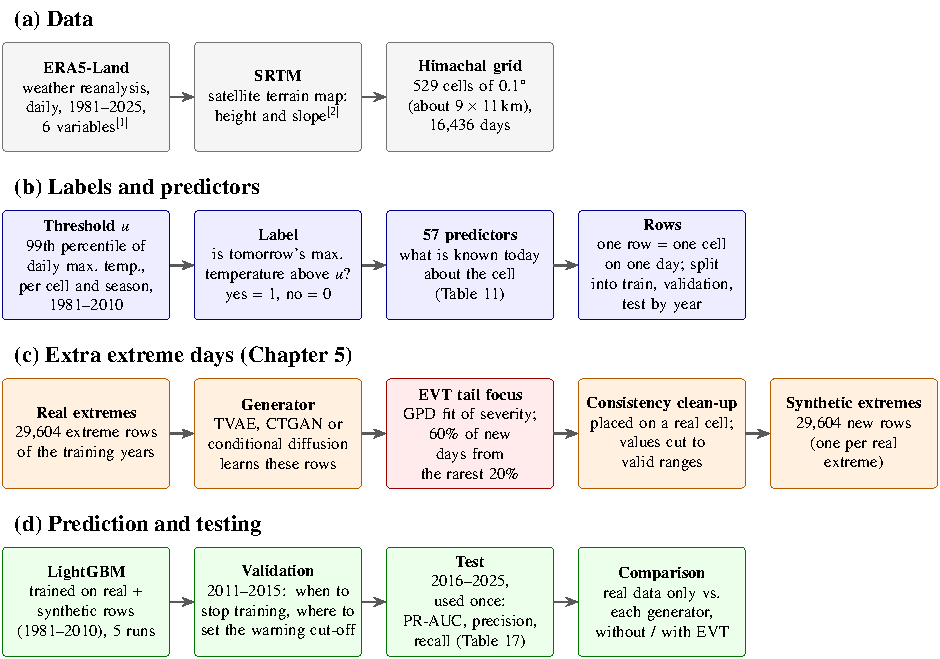
\includegraphics{diagram1.pdf}
\caption{Overview of the study. (a) Data sources and grid; (b) how labels and predictors are built; (c) how extra
extreme days are made; (d) how the classifier is trained and tested. [1] daily maximum, minimum and mean temperature,
dewpoint, surface pressure, solar radiation, top-layer soil water and rain (Table~\ref{tab:vars}); [2] NASA Shuttle
Radar Topography Mission, 30\,m elevation data averaged over each grid cell.}
\label{fig:pipeline}
\end{figure}

\begin{table}[H]
\centering
\caption{The numbers used throughout this report and what they mean}
\label{tab:numbers}
\footnotesize
\begin{tabularx}{\textwidth}{|>{\raggedleft\arraybackslash}p{1.75cm}|X|>{\raggedright\arraybackslash}p{4.3cm}|}
\hline
\textbf{Number} & \textbf{Meaning} & \textbf{How it is obtained}\\ \hline
529 & Grid cells covering Himachal Pradesh, each $0.1^\circ\times0.1^\circ$ (about $9.4\times11.1$\,km) & Cells of the
  $31\times37=1{,}147$-cell download box whose centre lies inside the state boundary \\ \hline
16{,}436 & Days in the record, 1 January 1981 to 31 December 2025 & 45 years of daily data \\ \hline
4 & Seasons: winter (Dec--Feb), pre-monsoon (Mar--May), monsoon (Jun--Sep), post-monsoon (Oct--Nov) & India
  Meteorological Department convention \\ \hline
99th percentile & Threshold $u$ above which a day is an extreme heat day & Computed per cell and per season from
  1981--2010 only \\ \hline
2{,}116 & Number of thresholds & $529\text{ cells}\times4\text{ seasons}$ \\ \hline
57 & Predictors describing a cell on one day & Listed one by one in Table~\ref{tab:predictors} \\ \hline
2{,}889{,}927 & Training rows (cell-days) & A random half of all cell-days of 1981--2010 \\ \hline
29{,}604 & Extreme rows among the training rows (1.02\%) & Rows whose label is 1 \\ \hline
965{,}954 & Validation rows, 2011--2015 & All cell-days of those years \\ \hline
1{,}932{,}437 & Test rows, 2016--2025, of which 37{,}450 extreme (1.94\%) & All cell-days of those years \\ \hline
296{,}040 & Rows generated by TVAE or CTGAN before selection & $10\times29{,}604$ \\ \hline
88{,}812 & Rows kept per generator after clean-up and EVT selection & $3\times29{,}604$ \\ \hline
29{,}604 & Synthetic rows added to one training run & One per real extreme row, drawn from the 88{,}812 \\ \hline
60\% / 20\% & EVT tail focus: 60\% of the added days lie in the most severe 20\% of the tail & Section~\ref{sec:evtmodel},
  Eq.~\ref{eq:mix} \\ \hline
5 & Training runs (seeds) per method; results are their mean or their combined prediction & Removes the luck of a
  single run \\ \hline
\end{tabularx}
\end{table}

\section{Problem Statement}
\textbf{Extreme Value-Guided Deep Generative Models for Imbalanced Classification:} (1) treat the minority class as a
tail phenomenon; (2) use EVT to characterise and constrain the tail; (3) use generative models to augment the data;
(4) ensure the synthetic data are consistent with real extremes and test whether they help. Research question:
\emph{with one fixed classifier (LightGBM), which way of generating extra extreme days helps most, and what does EVT
add?}

\section{Beneficiaries (Intended Users)}
Disaster-management and health authorities (local heat warnings), farmers and apple growers, water and hydropower
planners, weather services (a light statistical layer on existing forecasts), and researchers working on any
imbalanced problem whose rare class is a tail (fraud, failures, floods).

% =============================================================================
\chapter{Market Research}
% =============================================================================
\section{Existing Products and Approaches}
\begin{itemize}
  \item \textbf{IMD heat-wave warnings:} in the hills, a heat wave needs a maximum of at least 30\,$^\circ$C and
        4.5--6.4\,$^\circ$C above normal at two or more stations; colour-coded district warnings up to five days
        ahead~\cite{bhan_imd}.
  \item \textbf{Numerical weather prediction:} physics models on supercomputers; still the most reliable for record
        extremes~\cite{zhang2025records}.
  \item \textbf{AI weather models} (GraphCast, Pangu-Weather, FuXi): fast, 0.25$^\circ$, but under-predict record
        heat~\cite{zhang2025records,lopezgomez2023heat}.
  \item \textbf{Classifiers with rebalancing} (class weights, SMOTE) and \textbf{synthetic-data libraries}
        (SDV~\cite{patki2016sdv}).
\end{itemize}

\section{Comparison with Existing Products/Technologies}
\begin{table}[H]
\centering
\caption{Existing approaches compared with this project}
\label{tab:market}
\footnotesize
\begin{tabularx}{\textwidth}{|p{2.6cm}|X|X|p{2.0cm}|}
\hline
\textbf{Approach} & \textbf{Rare, severe days} & \textbf{Limitation here} & \textbf{Compute}\\ \hline
IMD warnings & Expert rules & Station scale; fixed thresholds & Operational \\ \hline
NWP & Best for records & No local extreme label & Supercomputer \\ \hline
AI weather models & Under-predict records & Coarse; tuned for average skill & GPU \\ \hline
Classifier + SMOTE & Interpolation & Little gain for strong classifiers~\cite{elor2022smote} & Low \\ \hline
Generic generators & Learn the bulk & Ignore the tail; break physics & Medium \\ \hline
\textbf{This project} & \textbf{EVT tail focus} & Next-day, reanalysis data & Free Colab \\ \hline
\end{tabularx}
\end{table}

\section{Problems with Existing Alternatives}
Fixed absolute thresholds do not describe what is extreme at high-altitude cells; models trained for average skill
miss the tail; balancing rarely helps strong classifiers~\cite{elor2022smote}; generic generators ignore the tail and
often break physics; large models need resources beyond a student project.

\section{How Our Approach Differs}
Extremes are defined per cell and season; a fitted EVT model decides which severities to add and caps how far they go;
the same EVT focus works with any generator (or none); every synthetic day is placed on a real cell and cut to valid ranges; and everything runs on free
compute.

% =============================================================================
\chapter{Literature Review}
% =============================================================================
\section{Imbalanced Classification}
Remedies either weight the rare class more or resample. SMOTE~\cite{chawla2002smote} creates points between a rare
example $x_i$ and a rare neighbour $x_{nn}$:
\begin{equation}
  x_{\text{new}} = x_i + \lambda\,(x_{nn}-x_i),
\end{equation}
where $\lambda$ is a random number between 0 and 1, so the new point lies on the line joining the two.
Borderline-SMOTE~\cite{han2005borderline} and ADASYN~\cite{he2008adasyn} focus on hard examples. For strong
classifiers such as gradient-boosted trees, balancing seldom helps~\cite{elor2022smote}.

\section{Extreme Value Theory}
By the Pickands--Balkema--de Haan theorem~\cite{pickands1975,balkema1974}, the excess $Y=X-u$ over a high threshold $u$
follows a Generalized Pareto Distribution (GPD)~\cite{coles2001}:
\begin{equation}
  F_{\xi,\sigma}(y)=1-\left(1+\frac{\xi y}{\sigma}\right)^{-1/\xi},\qquad 0<y<\infty\ (\xi\ge0),\quad 0<y<-\sigma/\xi\ (\xi<0) .
  \label{eq:gpd}
\end{equation}
Here $F_{\xi,\sigma}(y)$ is the chance that an excess is at most $y$, the scale $\sigma$ sets how spread out the excesses are, and the shape $\xi$ sets the tail: $\xi<0$ bounded (expected for temperature), $\xi=0$ exponential, $\xi>0$ heavy.

\section{Generative Models for Tabular Data}
A generative adversarial network (GAN)~\cite{goodfellow2014gan} trains two networks against each other: a
\emph{generator}, which turns random noise into data, and a \emph{discriminator}, which tries to tell real data from
generated data. Each improves against the other until the generated data look real. A variational autoencoder
(VAE)~\cite{kingma2014vae} instead learns to compress each example into a short code and rebuild it; new examples are
made by decoding random codes. CTGAN and TVAE~\cite{xu2019ctgan} adapt GANs and VAEs to tables. Diffusion
models~\cite{ho2020ddpm} add random noise to the data step by step and train a network to predict, and so remove, the
added noise; new data are made by starting from pure noise and removing it step by step.
Diffusion is strong for tabular data~\cite{kotelnikov2023tabddpm} and for minority samples~\cite{dsouza2025overlap}.

\section{Extremes and Generative Models}
ExGAN~\cite{bhatia2021exgan} and evtGAN~\cite{boulaguiem2022evtgan} generate or simulate extremes; heavy-tailed
diffusion~\cite{pandey2025heavy} targets far tails. Few studies test whether EVT-consistent synthetic data improve a
downstream classifier, or compare generator families under one fixed classifier. This project does both, using EVT to
\emph{guide} which severities any generator adds.

% =============================================================================
\chapter{Weather and Climate of India}
\label{ch:climate}
% =============================================================================
This chapter gives the climate background needed to read the rest of the report: how weather differs across the
regions of India, which factors cause these differences, and where Himachal Pradesh fits.

\section{Weather and Climate}
\textbf{Weather} is the state of the atmosphere at a place on a given day: temperature, humidity, pressure, wind,
cloud and rain. \textbf{Climate} is the long-term average of the weather and its usual range, normally described over
a 30-year period. This project predicts \emph{weather} (tomorrow's maximum temperature being extreme) but defines
``extreme'' from \emph{climate} (the 1981--2010 record of each grid cell).

\section{Seasons of India}
The India Meteorological Department (IMD) divides the year into four seasons, which this project also uses
(Table~\ref{tab:imdseasons}).

\begin{table}[H]
\centering
\caption{The four IMD seasons and their typical weather.}
\label{tab:imdseasons}
\small
\begin{tabular}{|p{2.6cm}|p{2.4cm}|p{9.4cm}|}
\hline
\textbf{Season} & \textbf{Months} & \textbf{Typical weather}\\ \hline
Winter & Dec, Jan, Feb & Cold and mostly dry; snow and rain in the north-west from western disturbances; fog
over the northern plains.\\ \hline
Pre-monsoon (summer) & Mar, Apr, May & Rapid heating; hottest time of year in the north and centre; heatwaves,
dust storms and hot dry winds (\emph{loo}); thunderstorms in the east and south.\\ \hline
Southwest monsoon & Jun, Jul, Aug, Sep & Moist winds from the Indian Ocean bring most of the year's rain; about 75\%
of India's annual rainfall (868.6\,mm of 1{,}160.1\,mm, 1971--2020 normal)~\cite{imd2022normal}.\\ \hline
Post-monsoon & Oct, Nov & Monsoon withdraws; clear skies in the north; the northeast monsoon brings the main rains of
Tamil Nadu (October--December).\\ \hline
\end{tabular}
\end{table}

\section{Weather Regions of India}
India stretches over about 30 degrees of latitude, from the equatorial south to the high Himalaya, so its weather
varies strongly from region to region. Two common ways of dividing it are used here.

\textbf{IMD homogeneous regions.} For monsoon monitoring and forecasting, IMD groups its meteorological subdivisions
into four broad regions with similar rainfall: Northwest India, Central India, South Peninsula, and East \& Northeast
India (Figure~\ref{fig:indiaregions}). Their normal June--September rainfall ranges from 587.6\,mm in Northwest India
to 1{,}367.3\,mm in East \& Northeast India~\cite{imd2026monsoon}. Himachal Pradesh belongs to \textbf{Northwest
India}, the driest of the four in the monsoon and the one most affected by winter western disturbances and pre-monsoon
heat.

\begin{figure}[H]
\centering
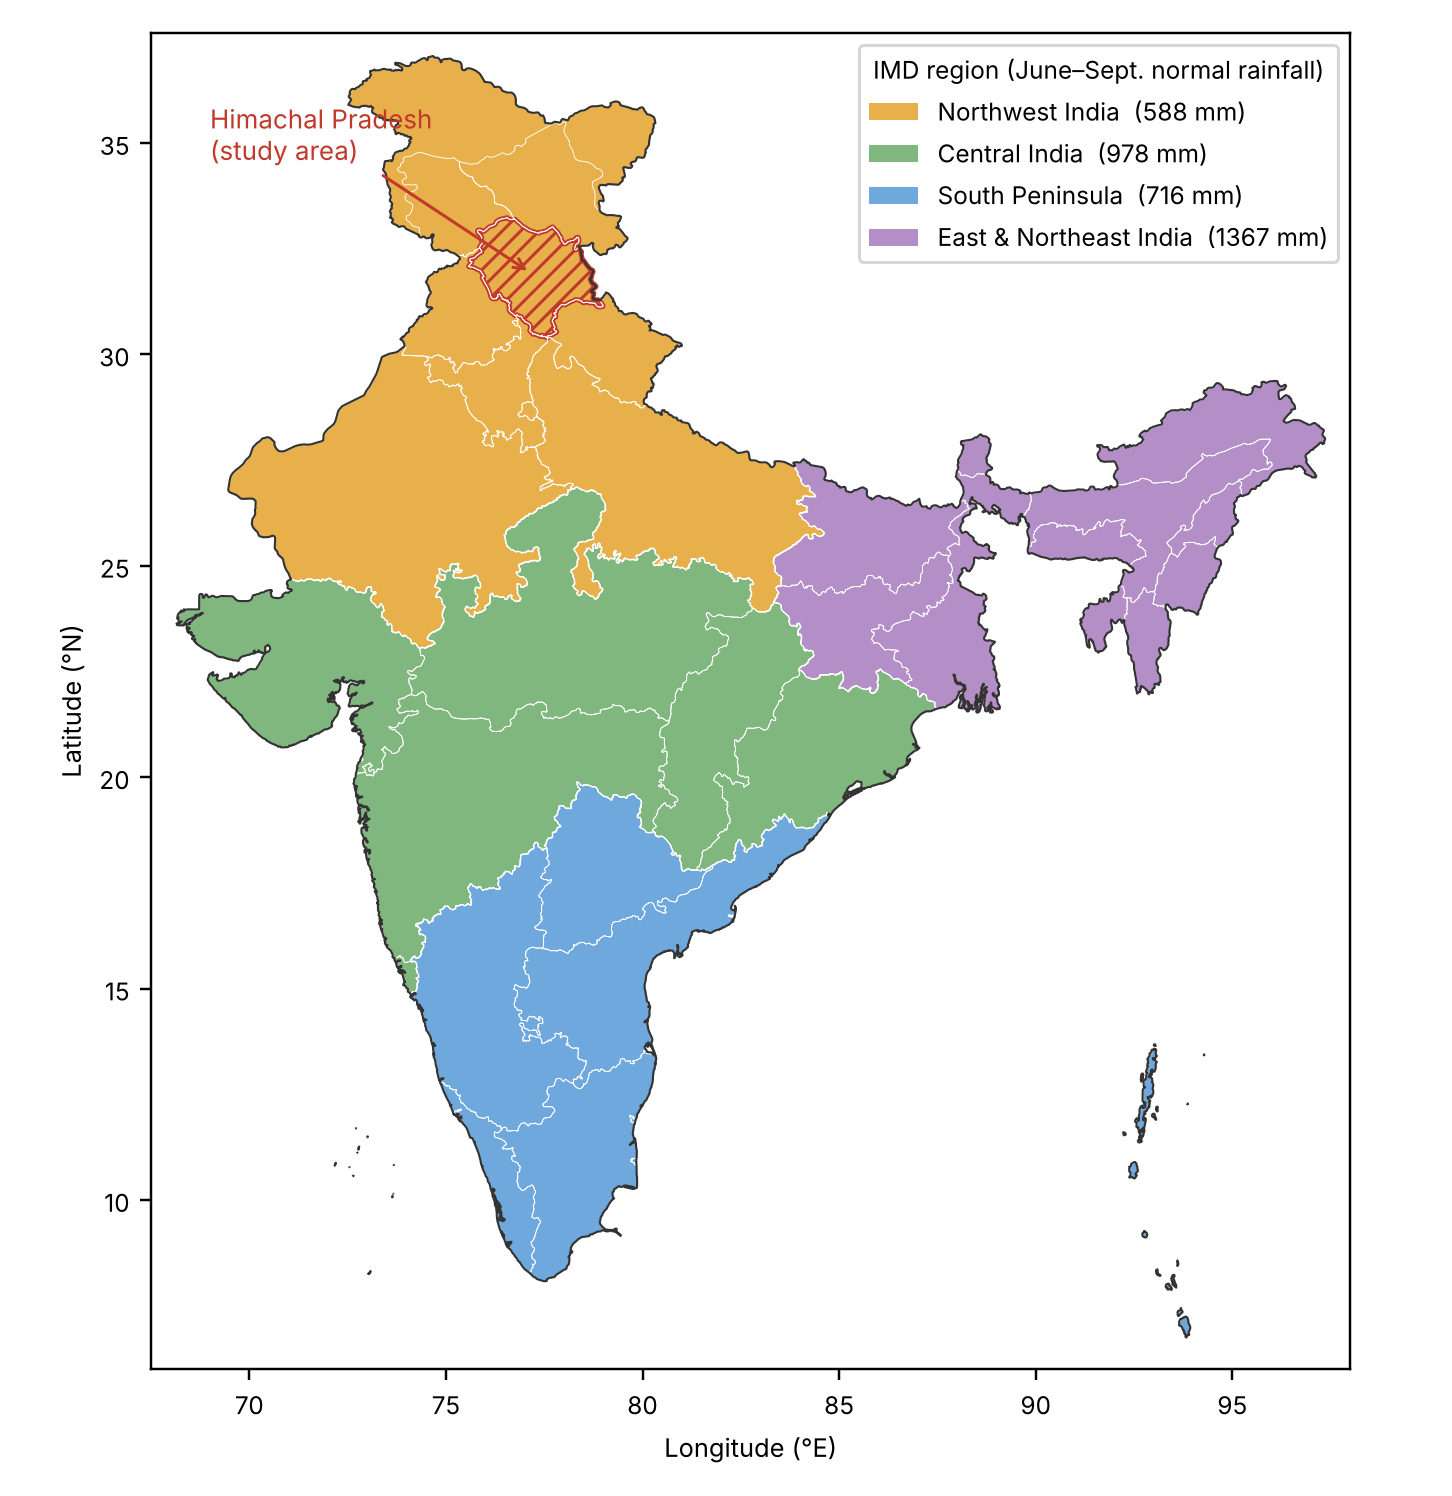
\includegraphics[width=0.74\textwidth]{fig_india_regions.png}
\caption{IMD's four homogeneous rainfall regions, drawn here by state, with their normal June--September rainfall
(1971--2020)~\cite{imd2026monsoon}. IMD defines the regions by meteorological subdivision, so the state outlines are
an approximation. Himachal Pradesh, the study area, is hatched. Boundaries: Natural Earth (India's official view)~\cite{naturalearth}.}
\label{fig:indiaregions}
\end{figure}

\textbf{Climate types.} By temperature and rainfall, the country also falls into a few broad climate types
(Figure~\ref{fig:indiaclimate} and Table~\ref{tab:climtypes}).

\begin{figure}[H]
\centering
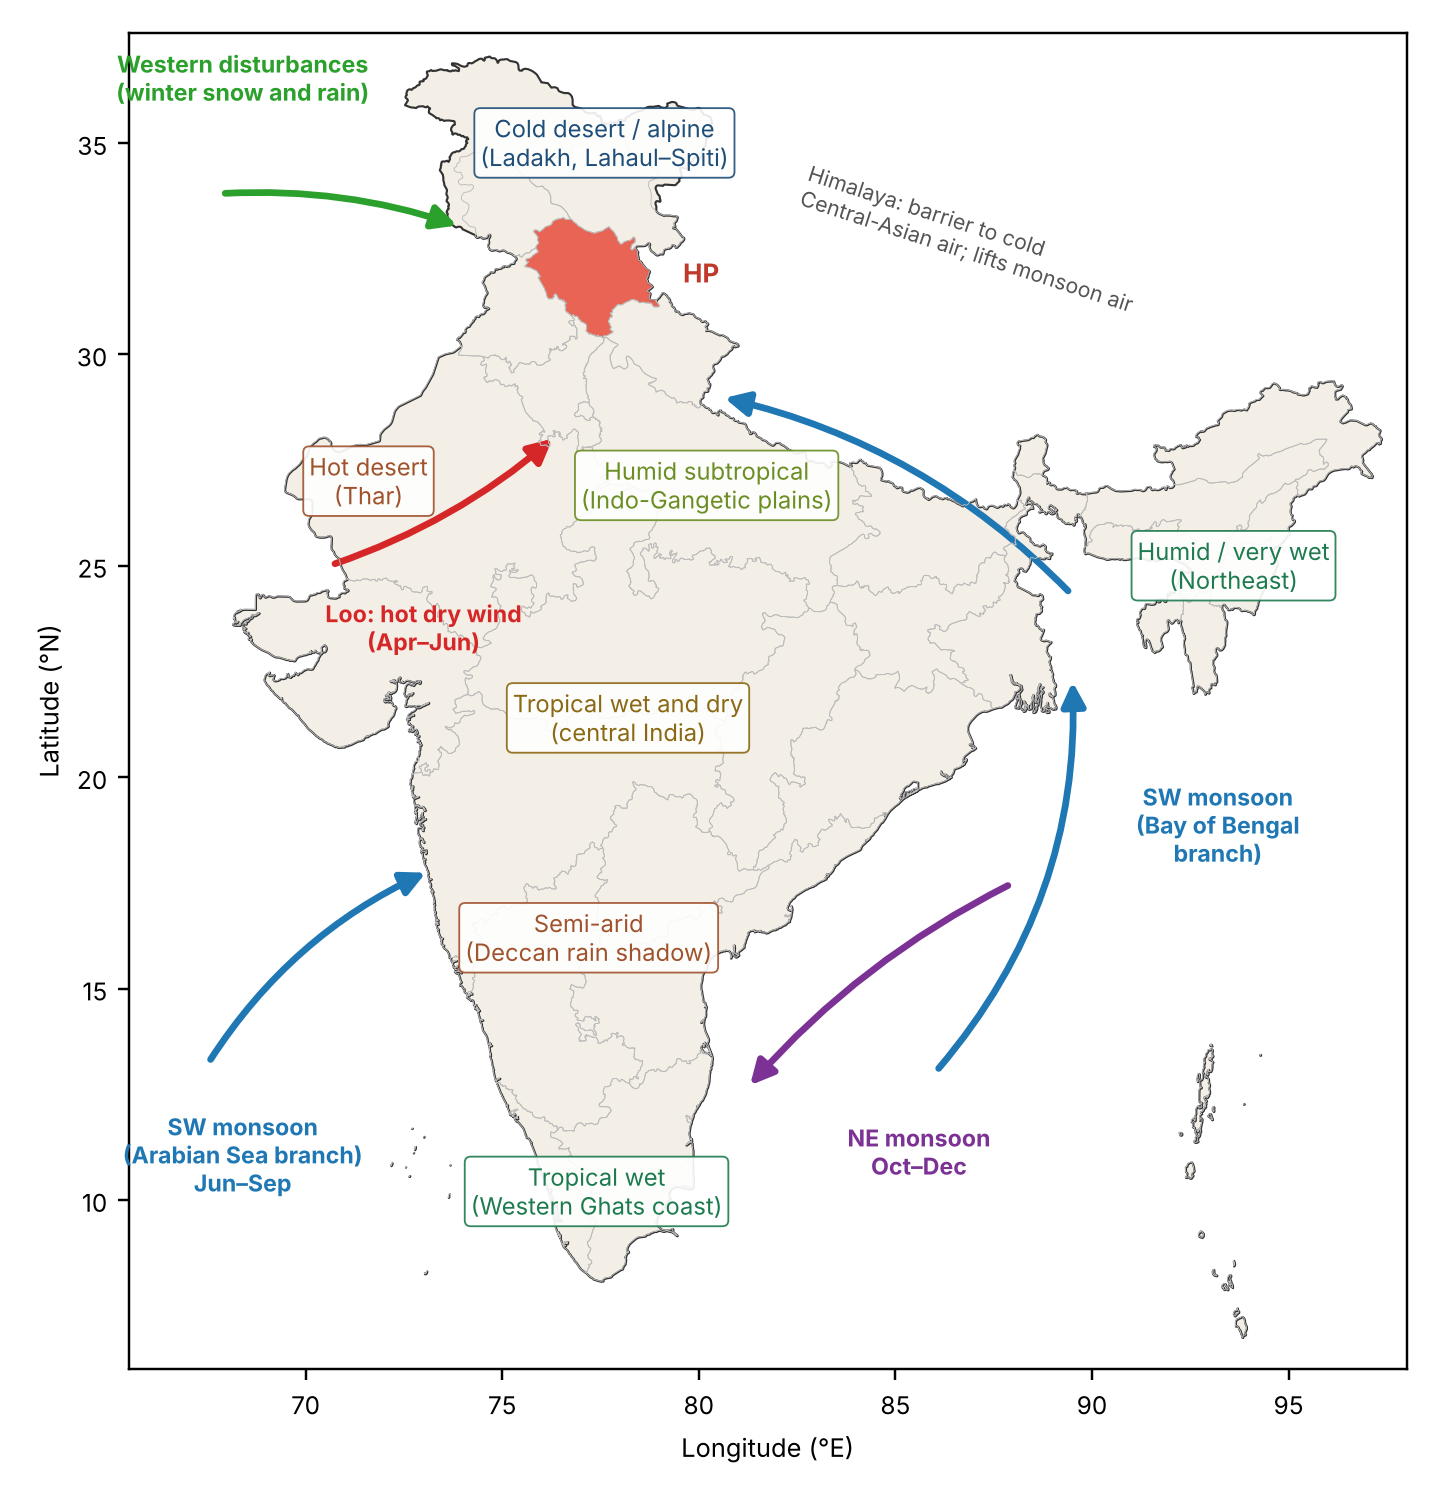
\includegraphics[width=0.74\textwidth]{fig_india_climate.png}
\caption{Broad climate types of India (labels placed at their typical location; no exact borders are implied) and
the main winds that shape them. Blue: the two branches of the southwest monsoon; purple: the northeast monsoon; green:
western disturbances; red: the hot \emph{loo} wind. Himachal Pradesh is shown in red.}
\label{fig:indiaclimate}
\end{figure}

\begin{table}[H]
\centering
\caption{Broad climate types of India.}
\label{tab:climtypes}
\small
\begin{tabular}{|p{3.2cm}|p{4.2cm}|p{7.0cm}|}
\hline
\textbf{Climate type} & \textbf{Where} & \textbf{Main features}\\ \hline
Tropical wet & Western Ghats coast (Kerala, Konkan), parts of the Northeast & Hot and humid all year; very heavy
monsoon rain on slopes facing the wind.\\ \hline
Tropical wet and dry & Most of central and peninsular India & Hot summers, a clear wet season (monsoon) and a long dry
season.\\ \hline
Semi-arid & Interior Deccan (in the rain shadow of the Western Ghats), parts of Gujarat and Rajasthan & Low, unreliable
rain; hot summers.\\ \hline
Hot desert & Thar desert (western Rajasthan) & Very little rain; very hot days and cool nights; dust storms.\\ \hline
Humid subtropical & Indo-Gangetic plains, Himalayan foothills (including lower Himachal Pradesh) & Hot summers with
heatwaves, wet monsoon, cool to cold winters with fog.\\ \hline
Mountain (temperate to alpine) & Himalaya (middle and high Himachal Pradesh, Uttarakhand, Jammu \& Kashmir, Sikkim)
& Temperature falls with height; winter snow; climate changes over short distances.\\ \hline
Cold desert & Ladakh, Lahaul--Spiti and upper Kinnaur & Behind the main Himalayan ranges; very dry, very cold
winters, strong sunshine.\\ \hline
\end{tabular}
\end{table}

\section{Factors that Affect Weather in India}
The regional differences above come from a small set of physical factors (Figure~\ref{fig:factors}).

\begin{figure}[H]
\centering
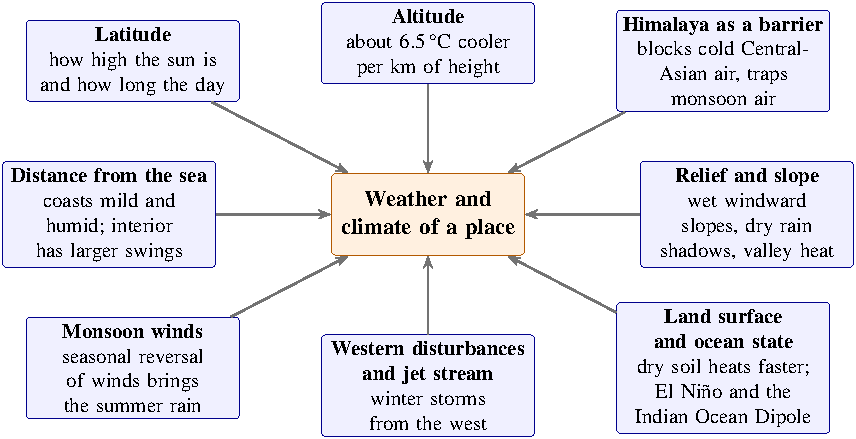
\includegraphics{diagram2.pdf}
\caption{The main factors that control the weather and climate of a place in India.}
\label{fig:factors}
\end{figure}

\begin{enumerate}
\item \textbf{Latitude.} The Tropic of Cancer crosses the middle of India. The south is close to the equator and warm
all year; the north has a large difference between summer and winter.
\item \textbf{Altitude.} Air cools by about 6.5\,$^\circ$C for each kilometre of height on average. This is why the
same calendar day can be 40\,$^\circ$C in the plains and below freezing in the high Himalaya, and why this project
sets a separate threshold for every grid cell (Figure~\ref{fig:thr}).
\item \textbf{The Himalaya as a barrier.} The mountain wall keeps the cold, dry winter air of Central Asia out of
northern India, and in summer forces the moist monsoon winds to rise and release their rain on the southern slopes.
\item \textbf{Distance from the sea.} The sea warms and cools slowly, so coastal places have small daily and yearly
temperature ranges and high humidity. Inland places, far from the sea, have hotter summers and colder winters.
\item \textbf{Relief and slope (orographic effect).} When moist air is pushed up a mountain it cools, its water
vapour condenses and rain falls on the windward side; the air that comes down the other side is dry and warm, leaving
a \emph{rain shadow} (Figure~\ref{fig:orographic}). The Western Ghats and the Deccan, and the main Himalayan ranges
and Lahaul--Spiti, are two such pairs.
\item \textbf{Monsoon winds.} In summer the land heats much faster than the Indian Ocean; low pressure over north-west
India draws in moist south-westerly winds from the sea (the \emph{southwest monsoon}, with an Arabian Sea branch and a
Bay of Bengal branch). In winter the winds reverse and blow from the land (the \emph{northeast monsoon}), giving rain
only where they cross the Bay of Bengal, mainly in Tamil Nadu.
\item \textbf{Western disturbances and the jet stream.} In winter and spring, storms that form over the Mediterranean
region travel east along the subtropical westerly jet stream and bring snow and rain to the western Himalaya. They are
the main source of winter precipitation in Himachal Pradesh.
\item \textbf{Land surface and ocean state.} Dry soil uses less of the sun's energy for evaporation, so more of it
heats the air: dry spells before or during the summer make heat extremes more likely. On a larger scale, El Ni\~no
events in the Pacific and the Indian Ocean Dipole change the strength of the monsoon from year to year.
\end{enumerate}

\begin{figure}[H]
\centering
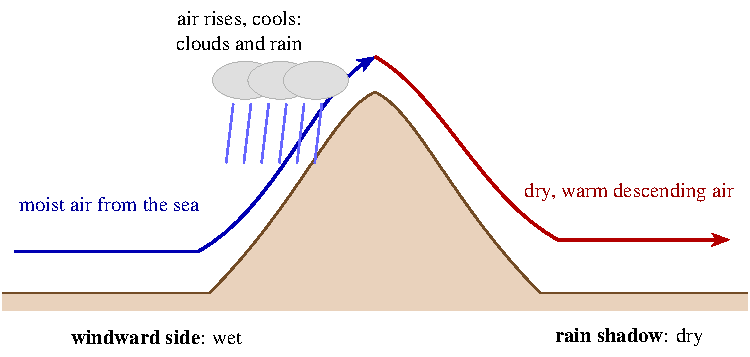
\includegraphics{diagram3.pdf}
\caption{The orographic effect: mountains make one side wet and the other dry.}
\label{fig:orographic}
\end{figure}

\section{Himachal Pradesh}
Himachal Pradesh lies in Northwest India on the southern side of the western Himalaya. Its height rises from about
300\,m near Una in the south-west to above 6{,}000\,m in the north-east, so it holds several climates within a short
distance. Using the elevation bands of the state's agro-climatic zones, the 529 grid cells of this project fall into
four groups (Figure~\ref{fig:hpzones}): 95 sub-tropical low-hill cells (below 1{,}000\,m), 47 sub-temperate mid-hill
cells (1{,}000--1{,}500\,m), 89 wet temperate high-hill cells (1{,}500--2{,}500\,m) and 298 dry temperate or cold-desert
cells (above 2{,}500\,m). More than half of the state therefore lies above 2{,}500\,m.

\begin{figure}[H]
\centering
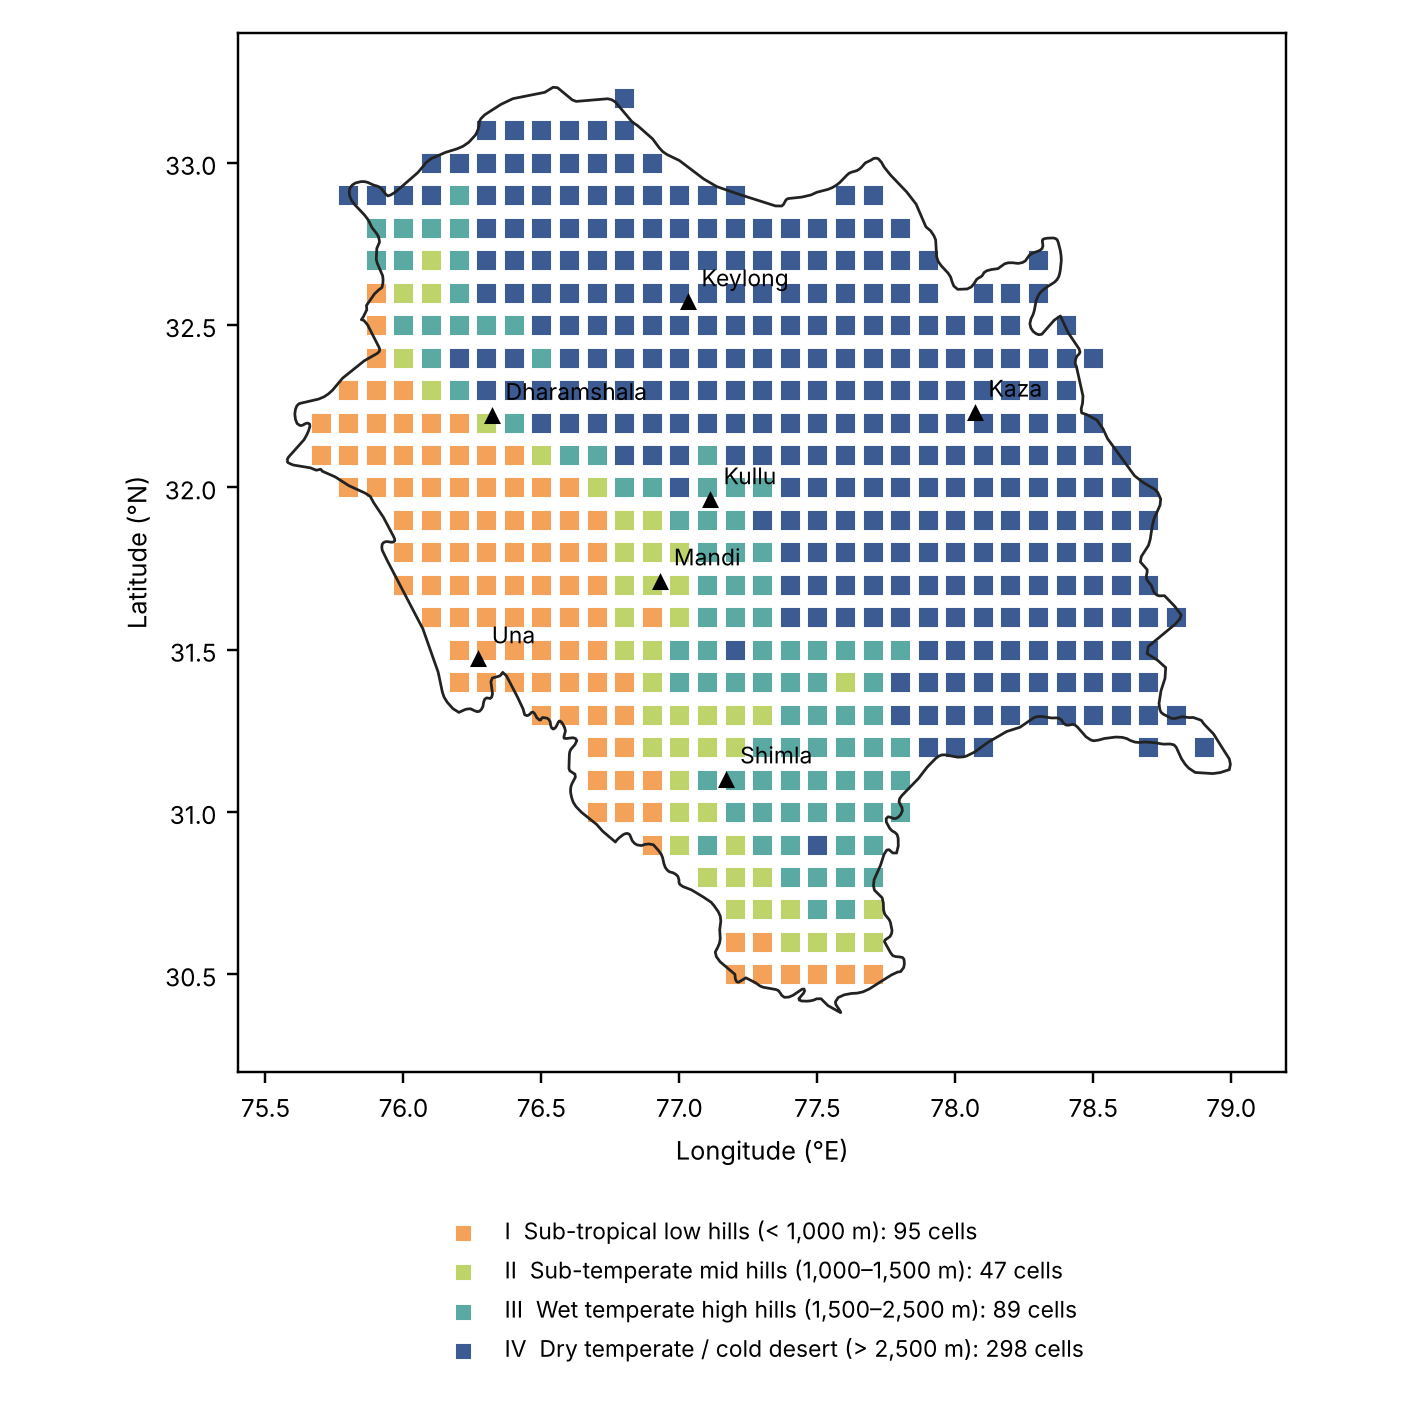
\includegraphics[width=0.66\textwidth]{fig_hp_zones.png}
\caption{The 529 grid cells of Himachal Pradesh coloured by elevation band (mean SRTM height of the cell). Triangles
mark towns for orientation.}
\label{fig:hpzones}
\end{figure}

\begin{itemize}
\item \textbf{Low hills (Una, Kangra valley, Bilaspur).} Hot pre-monsoon months with temperatures near those of the
Punjab plains, and a wet monsoon. Heatwaves from the plains reach here.
\item \textbf{Mid and high hills (Mandi, Shimla, Kullu).} Mild summers and cold winters with snow at higher places;
the heaviest monsoon rain falls on the outer ranges such as the Dhauladhar near Dharamshala.
\item \textbf{Cold desert (Lahaul--Spiti, upper Kinnaur).} Behind the Pir Panjal and Great Himalayan ranges, in their
rain shadow: little monsoon rain, snow mainly from western disturbances, very cold winters.
\end{itemize}

\textbf{Why this matters for the project.}
\begin{itemize}
\item The same temperature is ordinary in Una and extreme in Kaza, so a single national rule cannot describe extremes
everywhere. IMD itself uses different heatwave rules for plains (at least 40\,$^\circ$C) and hilly regions (at least
30\,$^\circ$C), together with a departure from normal of 4.5--6.4\,$^\circ$C (more than 6.4\,$^\circ$C is a severe heat
wave)~\cite{imdheatdef}, the same rule as quoted in Chapter~2. This project goes
one step further and uses the 99th percentile of each cell in each season (Section~\ref{sec:features}).
\item Seasons behave differently: pre-monsoon extremes are dry heat; monsoon extremes come in breaks of the monsoon;
winter extremes are warm spells between western disturbances. That is why thresholds and the EVT fit are computed per
season.
\item The factors above are what the predictors measure: elevation and slope (altitude and relief), soil moisture and
recent rain (land-surface dryness), humidity and dewpoint (monsoon moisture), surface pressure and its change
(passing disturbances) and solar radiation (clear skies).
\end{itemize}

% =============================================================================
\chapter{Data and Methodology}
\label{ch:method}
% =============================================================================
\section{Study Area and Data}
\subsection{Region of interest}
The study covers Himachal Pradesh, a mountain state of about 55{,}700\,km$^2$ in the western Himalaya, whose land rises
from about 300\,m in the south-west to more than 6{,}000\,m in the north-east (Figure~\ref{fig:area}). The state is
represented by a regular grid of $0.1^\circ\times0.1^\circ$ cells (about 9.4\,km east--west and 11.1\,km north--south
at $32^\circ$N, roughly 105\,km$^2$ each). The data were downloaded for the box 30.3--33.3$^\circ$N,
75.5--79.1$^\circ$E, which holds $31\times37=1{,}147$ cells; a cell is kept when its centre lies inside the state
boundary (GADM version 4.1). This leaves \textbf{529 cells}, covering about 55{,}500\,km$^2$, close to the area of the
state. Every result in this report is computed on these 529 cells for each day from 1 January 1981 to 31 December
2025 (16{,}436 days).

\begin{figure}[H]
\centering
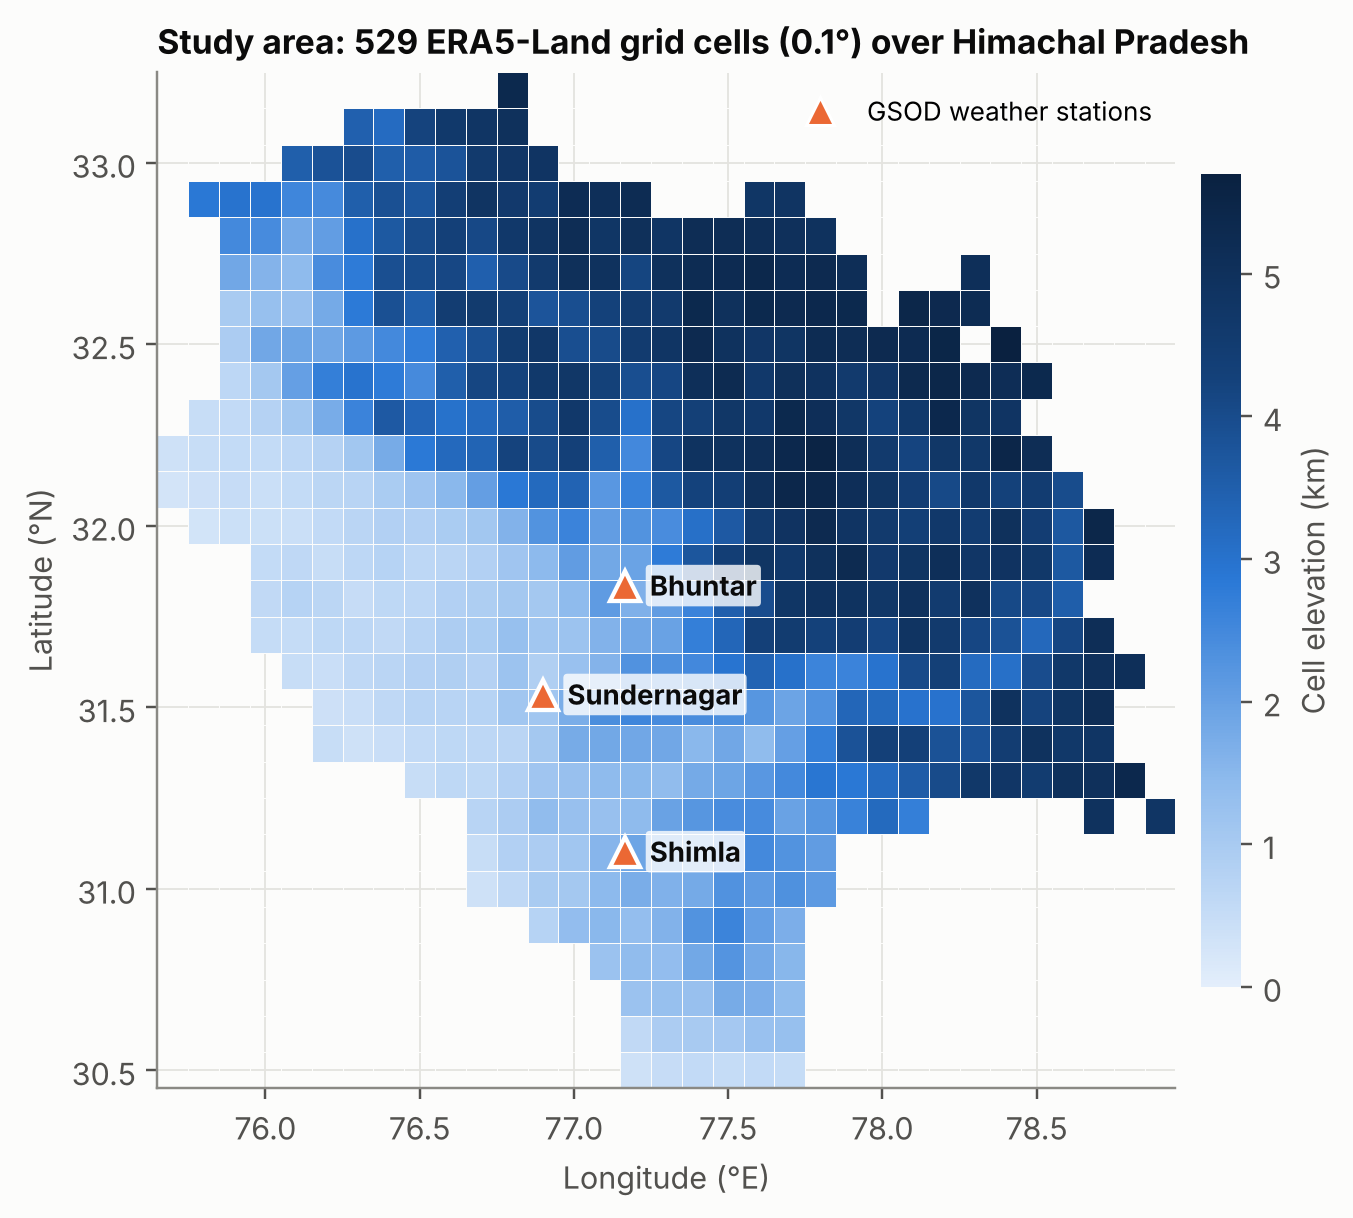
\includegraphics[width=0.75\textwidth]{fig_study_area.png}
\caption{Study area: the 529 grid cells coloured by mean elevation (from SRTM), with the three weather stations of the
GSOD archive in the state}
\label{fig:area}
\end{figure}

\subsection{Data sources}
Two data sets provide all model inputs; a third provides the state boundary (Table~\ref{tab:sources}).

\textbf{ERA5-Land}~\cite{munoz2021era5land} is a \emph{reanalysis} of the land surface produced by the European Centre
for Medium-Range Weather Forecasts (ECMWF) for the Copernicus Climate Change Service of the European Union. A
reanalysis re-runs a weather model over past decades while continuously correcting it with millions of real
observations (stations, satellites, balloons), and stores the result on a regular grid. The output is therefore a
complete, gap-free reconstruction of past weather: every cell has a value for every hour, even where no station
exists. ERA5-Land has a grid spacing of $0.1^\circ$, hourly values from 1950 to a few days before the present, and is
free to download from the Copernicus Climate Data Store. This study uses its daily statistics (daily maximum, minimum
and mean of the hourly values) for 1981--2025.

\textbf{SRTM}~\cite{farr2007srtm} (Shuttle Radar Topography Mission) is a digital elevation map of the Earth measured by
radar from the Space Shuttle \emph{Endeavour} in February 2000 by NASA. It gives the height of the ground every 30\,m.
For each grid cell the 30\,m heights were averaged to give the cell's \emph{mean elevation}, and the local slopes were
averaged to give its \emph{mean slope}. SRTM is used only for these two fixed (time-independent) predictors.

\begin{table}[H]
\centering
\caption{Data sources used}
\label{tab:sources}
\footnotesize
\begin{tabularx}{\textwidth}{|>{\raggedright\arraybackslash}p{2.0cm}|>{\raggedright\arraybackslash}X|>{\raggedright\arraybackslash}p{2.6cm}|>{\raggedright\arraybackslash}p{3.7cm}|}
\hline
\textbf{Data set} & \textbf{What it is} & \textbf{Resolution, period} & \textbf{Used for}\\ \hline
ERA5-Land & Reanalysis of past land-surface weather (ECMWF / Copernicus): a weather model corrected with observations &
  $0.1^\circ$ ($\approx$9\,km), hourly; 1981--2025 used & Daily weather of every cell (Table~\ref{tab:vars}); the
  labels \\ \hline
SRTM & Radar map of ground height (NASA, February 2000) & 30\,m, one fixed map & Mean elevation and mean slope of
  every cell \\ \hline
GADM 4.1 & Database of administrative boundaries & Vector outline & Which cells lie inside Himachal Pradesh \\ \hline
\end{tabularx}
\end{table}

\subsection{Why ERA5-Land, and the Data Sets Not Used}
The data had to meet five needs. (1)~\emph{Long record}: extreme days are about 1\% of days, so decades are needed to
have enough of them, plus a fixed 1981--2010 baseline and unseen test years up to 2025. (2)~\emph{Fine grid}:
Himachal rises from 300\,m to over 6\,km, and a valley and a ridge 20\,km apart have very different climates.
(3)~\emph{No gaps}: every cell must have every day. (4)~\emph{Many variables}: humidity, soil moisture, radiation and
rain, not only temperature. (5)~\emph{Free and still updated}. ERA5-Land is the only option found that meets all five.
Table~\ref{tab:datasets} lists the other data sets that were considered.

\begin{table}[H]
\centering
\caption{Data sets considered for the study}
\label{tab:datasets}
\footnotesize
\begin{tabularx}{\textwidth}{|>{\raggedright\arraybackslash}p{2.5cm}|>{\raggedright\arraybackslash}p{2.6cm}|>{\raggedright\arraybackslash}p{2.0cm}|>{\raggedright\arraybackslash}X|}
\hline
\textbf{Data set} & \textbf{Grid / coverage} & \textbf{Period} & \textbf{Why not used}\\ \hline
\textbf{ERA5-Land}~\cite{munoz2021era5land} (chosen) & 0.1$^\circ$ ($\approx$9\,km), 529 cells & 1950--now & Used: long, fine,
  gap-free, many variables \\ \hline
ERA5~\cite{hersbach2020era5} & 0.25$^\circ$ ($\approx$28\,km), $\approx$85 cells & 1940--now & Too coarse: valleys and
  ridges fall in the same cell; ERA5-Land is its finer land version \\ \hline
IMD gridded temperature~\cite{srivastava2009imd} & 1$^\circ$, fewer than 10 cells & 1951--now & Far too coarse;
  interpolated from few hill stations; temperature only \\ \hline
IMDAA~\cite{rani2021imdaa} & 12\,km & 1979--2018 at release & Does not cover the test years up to 2025 \\ \hline
MERRA-2~\cite{gelaro2017merra2} & 0.5$^\circ\times$0.625$^\circ$ & 1980--now & Too coarse for mountains \\ \hline
GSOD stations~\cite{gsod} & Points; 3 usable in the state & 2000--2025 checked & Only 3 stations (Shimla,
  Sundernagar, Bhuntar), 33--72\% of days present, about 9 usable years each; too few extremes to train on.
  Kept as a reference for later checks \\ \hline
CMIP6 climate models~\cite{eyring2016cmip6} & $\approx$100\,km & Simulated & Simulated weather, not the real days, so it
  cannot be used to predict a real tomorrow \\ \hline
\end{tabularx}
\end{table}

\noindent ERA5-Land is a model reconstruction, not a measurement, and can be biased in steep terrain. The labels are
therefore relative to each cell's own climate (its own 99th percentile), which reduces the effect of a constant bias,
and checking the severe days against stations is left as future work.

\subsection{ERA5-Land Variables Used}
ERA5-Land provides about 50 variables~\cite{munoz2021era5land}. Only those with a clear link to surface heat were
downloaded, which kept the data small enough for free cloud computing (Table~\ref{tab:vars}). Six ERA5-Land variables were used
(temperature counts once, with its three daily statistics); snow depth was downloaded but dropped, because glacier cells hold a fixed placeholder of 10\,m water equivalent.
Relative humidity was computed from temperature and dewpoint (Magnus formula), and elevation and slope come from SRTM
terrain, not ERA5-Land. Temperatures were converted from
kelvin to $^\circ$C, pressure from Pa to hPa, rain from m to mm, and radiation from J\,m$^{-2}$ per day to
W\,m$^{-2}$; rain and radiation, which ERA5-Land stamps at midnight of the next day, were moved back to the day they
belong to. The raw (not bias-corrected) ERA5-Land values are used. All 57 predictors
(Table~\ref{tab:predictors}) are built from these variables and the two SRTM terrain values.

\begin{table}[H]
\centering
\caption{ERA5-Land variables considered, with the units used in this report}
\label{tab:vars}
\footnotesize
\begin{tabularx}{\textwidth}{|>{\raggedright\arraybackslash}p{4.0cm}|>{\raggedright\arraybackslash}p{1.3cm}|>{\raggedright\arraybackslash}p{1.55cm}|>{\raggedright\arraybackslash}p{1.6cm}|>{\raggedright\arraybackslash}X|}
\hline
\textbf{Variable} & \textbf{Code} & \textbf{Unit} & \textbf{Status} & \textbf{Why}\\ \hline
2\,m air temperature: daily maximum, minimum, mean & \texttt{t2m\_max}, \texttt{t2m\_min}, \texttt{t2m\_mean} &
  $^\circ$C & Used & The heat signal itself; the daily maximum also defines the label\\ \hline
2\,m dewpoint temperature, daily mean & \texttt{d2m} & $^\circ$C & Used & Moisture in the air\\ \hline
Relative humidity (computed) & \texttt{rh} & \% & Used & From mean temperature and dewpoint (Magnus formula)\\ \hline
Surface pressure, daily mean & \texttt{sp} & hPa & Used & Rising pressure marks settled, clear weather\\ \hline
Surface solar radiation downwards, daily mean & \texttt{ssrd} & W\,m$^{-2}$ & Used & Sunshine reaching the ground\\ \hline
Soil water, top layer (0--7\,cm) & \texttt{swvl1} & m$^3$\,m$^{-3}$ & Used & Dry soil turns more sunshine into heat\\ \hline
Total precipitation, daily total & \texttt{tp} & mm & Used & Rain cools the surface; dry spells come before
  heatwaves\\ \hline
Snow depth & \texttt{sd} & m water & Dropped & Glacier cells stuck at a 10\,m placeholder\\ \hline
10\,m wind ($u$, $v$, speed) & \texttt{u10}, \texttt{v10} & m\,s$^{-1}$ & In file, not used & Daily-mean wind
  over steep terrain is a weak, indirect signal for next-day heat\\ \hline
Evaporation, skin temperature, runoff, deeper soil layers, thermal radiation, leaf area, others & -- & --
  & Not downloaded & Weaker or indirect link to next-day heat; kept the data within free computing limits\\ \hline
\end{tabularx}
\end{table}

% =============================================================================
\section{Data Processing and Quality Checks}
\label{sec:processing}
Before any model was built, the downloaded data were assembled into one file, checked against the original
ERA5-Land files, repaired where needed, and turned into model rows in three versions. This section records that
work, because every later result depends on it. All checks only read the data; repairs were written to new files.

\subsection{From downloads to one data file}
ERA5-Land daily statistics were downloaded from the Copernicus Climate Data Store one variable and one year at a
time for the box 30.3--33.3$^\circ$N, 75.5--79.1$^\circ$E. They were merged into a single file covering 16{,}436 days
(1 January 1981 to 31 December 2025) on the $31\times37$ grid, with 15 daily variables. Besides the variables of
Table~\ref{tab:vars}, the file also held 10\,m wind ($u$, $v$ and speed), the daily temperature range, and CHIRPS
satellite--gauge rainfall~\cite{funk2015chirps}; these were not used as predictors (the temperature range repeats
maximum minus minimum, and ERA5-Land rain was kept so that all predictors come from one consistent source). Static
layers were added: mean SRTM elevation and slope of each cell, and a mask marking the 529 cells whose centre lies in
Himachal Pradesh.

\subsection{Check against the original files}
A read-only check (Table~\ref{tab:qc}) compared the merged file with the original ERA5-Land files at five cells from
522\,m to 5{,}279\,m and six sample years (1981, 1990, 1991, 2005, 2020, 2025), and checked completeness and physical
consistency over all 529 cells and all days.

\begin{table}[H]
\centering
\caption{Quality checks on the merged data file (Himachal cells, 1981--2025)}
\label{tab:qc}
\footnotesize
\begin{tabularx}{\textwidth}{|>{\raggedright\arraybackslash}p{3.6cm}|>{\raggedright\arraybackslash}X|>{\raggedright\arraybackslash}p{4.4cm}|}
\hline
\textbf{Check} & \textbf{Result} & \textbf{Action}\\ \hline
Daily max, min, mean temperature and dewpoint vs original files & Identical after subtracting 273.15 (kelvin to
$^\circ$C), same day; largest difference 0.00 & None\\ \hline
Soil water and snow depth vs original & Identical & None\\ \hline
Rain vs original & Identical after $\times1000$ (m to mm) \emph{and a shift of one day}: ERA5-Land stamps a day's
total at 00\,UTC of the next day & Rain moved back to its own day\\ \hline
Pressure and solar radiation & Ranges 497--986\,hPa and 8--414\,W\,m$^{-2}$, consistent with Pa$\to$hPa and daily
J\,m$^{-2}\to$ W\,m$^{-2}$ (radiation also shifted one day) & None\\ \hline
Completeness & 100\% of cell-days for every variable and year, except daily mean temperature and humidity: empty for
1981--1985 although the original files were complete & Refilled from the original files; humidity recomputed
(Section~\ref{sec:repairs})\\ \hline
Snow depth & 6 of 529 cells (glaciers, 5{,}122--5{,}552\,m) stuck at 10\,m water equivalent on most days & Snow depth
dropped\\ \hline
Physical consistency & Minimum above maximum: 0 of 8{,}694{,}644 cell-days. Mean outside [min, max] by more than
0.5\,$^\circ$C: 0 of 7{,}728{,}690. Maximum temperature from $-36.6$ to $45.5\,^\circ$C & None\\ \hline
Label idea & Share of cell-days above each cell's own 99th percentile of maximum temperature: 1.00\% & Basis of the
labels\\ \hline
\end{tabularx}
\end{table}

\subsection{Repairs}
\label{sec:repairs}
Daily mean temperature for 1981--1985 was copied from the original ERA5-Land files (365 or 366 days per year), after
which no variable had a missing value. Relative humidity was recomputed for all years from mean temperature $T$ and
dewpoint $T_d$ with the standard Magnus formula (constants $a=17.625$ and $b=243.04\,^\circ$C); where the old file had humidity, the recomputed values differed by at most 0.03 percentage points.

\subsection{Weather stations as a reference}
To see whether station records could serve as ground truth, all NOAA GSOD stations~\cite{gsod} in the box were
checked for 2000--2025 (temperatures converted from $^\circ$F, missing values coded 9999.9 removed). Of 26 station
entries, 11 reported any data, and only three inside the state had at least eight years with 80\% of days complete
(Table~\ref{tab:gsod}). This is far too few for a 529-cell study, so stations are used only as reference points
(Figure~\ref{fig:area}), not as labels.

\begin{table}[H]
\centering
\caption{GSOD stations in Himachal Pradesh with usable records, 2000--2025}
\label{tab:gsod}
\small
\begin{tabular}{|l|c|c|c|}
\hline
\textbf{Station} & \textbf{Elevation (m)} & \textbf{Days with max and min (\%)} & \textbf{Usable years ($\ge$80\% of days)}\\ \hline
Sundernagar & 874 & 71.9 & 8\\ \hline
Bhuntar (Kullu) & 1{,}084 & 34.9 & 9\\ \hline
Shimla & 2{,}202 & 33.0 & 9\\ \hline
\end{tabular}
\end{table}

\subsection{Three versions of the model rows}
The model rows were built three times, each fixing a problem found by the one before (Table~\ref{tab:versions}).

\begin{table}[H]
\centering
\caption{Versions of the model-ready data}
\label{tab:versions}
\footnotesize
\begin{tabularx}{\textwidth}{|>{\raggedright\arraybackslash}p{1.7cm}|>{\raggedright\arraybackslash}X|>{\raggedright\arraybackslash}X|}
\hline
\textbf{Version} & \textbf{What it contained} & \textbf{What it showed}\\ \hline
v1--v2 & 35 predictors (place, day of year, 9 weather values for 3 days, today's anomalies); six labels: heat and
cold extremes, each against the same season, the whole year, or the same time of year ($\pm7$ days); all
5{,}794{,}666 training rows & Whole-year labels put almost all heat extremes in May--August (0.00\% in
November--February), so a hot winter day never counted; season-wise labels give about 1\% in every season and were
kept. Cold extremes were left for future work\\ \hline
v2 + fixes & Standardised GPD fits; gap-to-threshold predictors added (how far today and the two days before are from
tomorrow's threshold) & Without them, persistence (0.586 test PR-AUC) beat LightGBM (0.434). They raised LightGBM to
0.531, and the day-of-year predictors were found to hurt (0.549 without them), so they were dropped\\ \hline
v3 (final) & 57 predictors (Table~\ref{tab:predictors}) with 7--30-day history; a random half of the 1981--2010 rows
(2{,}889{,}927) for training; severity $z$ and onset stored for scoring only & With 7--30-day history LightGBM on real data reached 0.599, above persistence; used for all results in
Chapter~\ref{ch:results}\\ \hline
\end{tabularx}
\end{table}

\subsection{What the processed data show}
Figure~\ref{fig:yearly} shows the share of extreme heat cell-days in each year. By construction it averages 1\% over
1981--2010 (1.02\% in the training years); it stays at 1.00\% in 2011--2015 and almost doubles to 1.94\% in
2016--2025, with peaks in 2016, 2020 and 2024. The most widespread single events were 6 October 1983 (522 of 529
cells extreme), 26 May 1984 (448 cells) and 4 December 1988 (383 cells).

\begin{figure}[H]
\centering
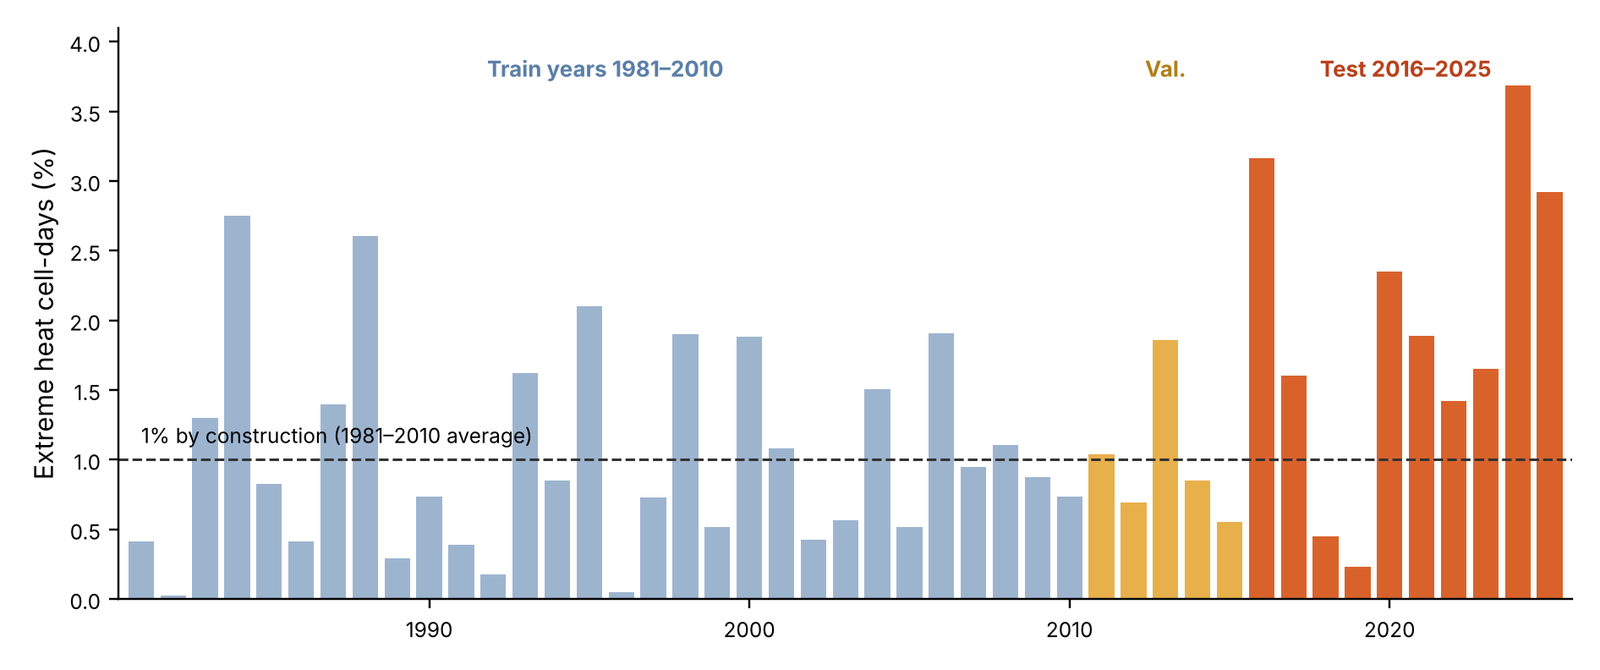
\includegraphics[width=0.95\textwidth]{fig_yearly_extremes.png}
\caption{Share of extreme heat cell-days per year (season-wise 99th-percentile labels, 529 cells). Dashed line: the
1\% that the 1981--2010 thresholds give by construction.}
\label{fig:yearly}
\end{figure}

\section{Extreme Heat Days, Predictors and Splits}
\label{sec:features}
\subsection{Seasons, thresholds and labels}
Each day belongs to one of four seasons, following the India Meteorological Department: winter (December--February),
pre-monsoon (March--May), monsoon (June--September) and post-monsoon (October--November). For cell $c$ and season $g$
the threshold $u_{c,g}$ is the 99th percentile of the daily maximum temperature $T^{\max}$ of that cell in that season,
computed from 1981--2010 only. This gives $529\times4=2{,}116$ thresholds. A day $t$ is an \emph{extreme heat day} if
\begin{equation}
  T^{\max}_{c,t}>u_{c,g(t)} ,
\end{equation}
so by construction about 1\% of the days of 1981--2010 are extreme in every cell and season. Because each cell is
compared with its own past, a hot day in a high valley and a hot day in the plains are both detected, although their
temperatures differ by more than 20\,$^\circ$C. Thresholds fall by about 5.5--8\,$^\circ$C per km of altitude, depending on the season
(Figure~\ref{fig:thr}). With the same fixed thresholds, extremes were almost twice as frequent in 2016--2025 as in
1981--2010 (1.94\% vs 1.02\% of cell-days).

\begin{figure}[H]
\centering
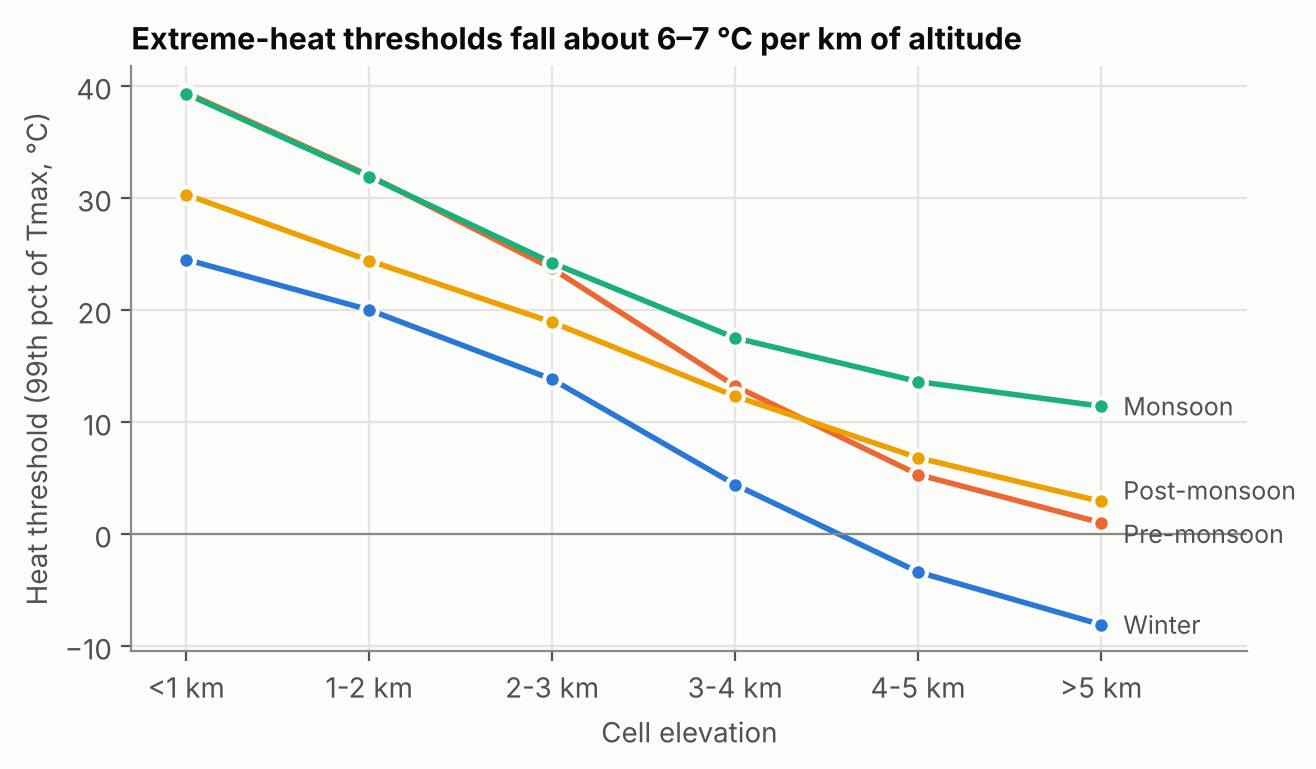
\includegraphics[width=0.75\textwidth]{fig_thresholds.png}
\caption{Mean extreme-heat threshold by elevation band and season}
\label{fig:thr}
\end{figure}

\noindent The prediction task is: \emph{given what is known on day $D$ (today), will day $D+1$ (tomorrow) be an
extreme heat day in this cell?} The label of a row is 1 if $D+1$ is extreme and 0 otherwise. The \emph{normal} used
below is the 1981--2010 mean of $T^{\max}$ (or $T^{\min}$) of the cell over the 15 days centred on the same calendar
day.

\subsection{The 57 predictors}
Each row describes one cell on one day $D$ with 57 numbers (Table~\ref{tab:predictors}), all known on day $D$: the place
(4), the weather of the last three days (27), today's departure from normal (2), summaries of the last one to four
weeks (16; two counters look further back, up to 60 and 365 days), and the distance between recent temperatures and tomorrow's threshold (8). Figure~\ref{fig:timeline} shows
which days each group looks at. The generators (Section~\ref{sec:arch}) produce the first 49 predictors; the last
eight are always recomputed from the cell's own threshold.

\begin{figure}[H]
\centering
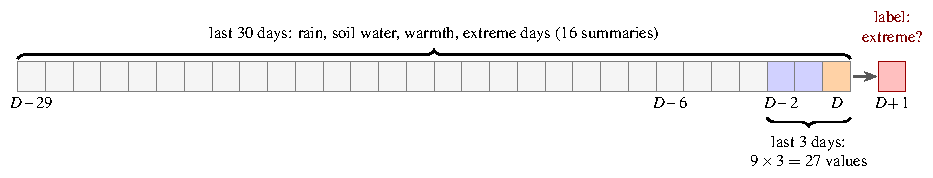
\includegraphics{diagram4.pdf}
\caption{Days used by one row. Today is day $D$ (orange); the predictors use only days up to $D$, and the label is
whether day $D+1$ is extreme. The 7- and 14-day summaries use the last 7 and 14 of the 30 days.}
\label{fig:timeline}
\end{figure}

{\footnotesize
\setlength{\LTpre}{4pt}\setlength{\LTpost}{4pt}
\begin{longtable}{|>{\raggedright\arraybackslash}p{3.3cm}|>{\raggedright\arraybackslash}p{6.0cm}|>{\raggedright\arraybackslash}p{1.55cm}|>{\raggedright\arraybackslash}p{2.2cm}|c|}
\caption{The 57 predictors of one row (cell $c$, day $D$). ``Normal'' is the 1981--2010 mean for the same calendar day
($\pm7$ days); $u$ is the threshold of tomorrow's season; $s$ is the cell's standard deviation of daily
$T^{\max}$ anomalies in that season.}\label{tab:predictors}\\
\hline
\textbf{Code} & \textbf{Meaning} & \textbf{Unit} & \textbf{Days used} & \textbf{No.}\\ \hline
\endfirsthead
\hline
\textbf{Code} & \textbf{Meaning} & \textbf{Unit} & \textbf{Days used} & \textbf{No.}\\ \hline
\endhead
\hline
\endfoot
\rowcolor{black!6}\multicolumn{5}{|l|}{\textbf{A. Place of the cell} (fixed; grid and SRTM)} \\ \hline
\texttt{lat}, \texttt{lon} & Latitude and longitude of the cell centre & $^\circ$N, $^\circ$E & -- & 2\\ \hline
\texttt{elev\_m} & Mean ground height of the cell (SRTM) & m & -- & 1\\ \hline
\texttt{slope\_deg} & Mean terrain slope of the cell (SRTM) & degrees & -- & 1\\ \hline
\rowcolor{black!6}\multicolumn{5}{|l|}{\textbf{B. Weather of the last three days} (ERA5-Land; suffix \texttt{\_l0},
  \texttt{\_l1}, \texttt{\_l2} = today, yesterday, day before)} \\ \hline
\texttt{t2m\_max\_l0..l2} & Daily maximum 2\,m air temperature & $^\circ$C & $D$, $D\!-\!1$, $D\!-\!2$ & 3\\ \hline
\texttt{t2m\_min\_l0..l2} & Daily minimum 2\,m air temperature & $^\circ$C & $D$, $D\!-\!1$, $D\!-\!2$ & 3\\ \hline
\texttt{t2m\_mean\_l0..l2} & Daily mean 2\,m air temperature & $^\circ$C & $D$, $D\!-\!1$, $D\!-\!2$ & 3\\ \hline
\texttt{d2m\_l0..l2} & Daily mean 2\,m dewpoint temperature & $^\circ$C & $D$, $D\!-\!1$, $D\!-\!2$ & 3\\ \hline
\texttt{rh\_l0..l2} & Relative humidity from mean temperature and dewpoint & \% & $D$, $D\!-\!1$, $D\!-\!2$ & 3\\ \hline
\texttt{sp\_l0..l2} & Daily mean surface pressure & hPa & $D$, $D\!-\!1$, $D\!-\!2$ & 3\\ \hline
\texttt{ssrd\_l0..l2} & Daily mean solar radiation reaching the ground & W\,m$^{-2}$ & $D$, $D\!-\!1$, $D\!-\!2$ & 3\\ \hline
\texttt{swvl1\_l0..l2} & Soil water in the top 7\,cm & m$^3$\,m$^{-3}$ & $D$, $D\!-\!1$, $D\!-\!2$ & 3\\ \hline
\texttt{tp\_l0..l2} & Daily total rain & mm & $D$, $D\!-\!1$, $D\!-\!2$ & 3\\ \hline
\rowcolor{black!6}\multicolumn{5}{|l|}{\textbf{C. Today compared with normal}} \\ \hline
\texttt{tmax\_anom\_l0} & Today's maximum temperature minus its normal & $^\circ$C & $D$ & 1\\ \hline
\texttt{tmin\_anom\_l0} & Today's minimum temperature minus its normal & $^\circ$C & $D$ & 1\\ \hline
\rowcolor{black!6}\multicolumn{5}{|l|}{\textbf{D. The last one to four weeks} (windows end on today; two counters look back up to 60 and 365 days)} \\ \hline
\texttt{tmax\_anom\_m7, m14, m30} & Mean maximum-temperature anomaly over the last 7, 14 and 30 days & $^\circ$C & up to
  30 days & 3\\ \hline
\texttt{tmin\_anom\_m7, m30} & Mean minimum-temperature anomaly over the last 7 and 30 days & $^\circ$C & up to 30
  days & 2\\ \hline
\texttt{warm\_spell\_days} & Consecutive days up to today with maximum temperature above normal (at most 60) & days &
  up to 60 days & 1\\ \hline
\texttt{days\_since\_extreme} & Days since the cell's last extreme heat day (at most 365) & days & up to 365 days &
  1\\ \hline
\texttt{extremes\_last30} & Number of extreme heat days in the last 30 days & count & 30 days & 1\\ \hline
\texttt{tp\_sum7, tp\_sum30} & Total rain over the last 7 and 30 days & mm & 7, 30 days & 2\\ \hline
\texttt{swvl1\_m14, m30} & Mean top-layer soil water over the last 14 and 30 days & m$^3$\,m$^{-3}$ & 14, 30 days &
  2\\ \hline
\texttt{swvl1\_change14} & Soil water today minus 14 days ago (drying is negative) & m$^3$\,m$^{-3}$ & $D$, $D\!-\!14$
  & 1\\ \hline
\texttt{d2m\_m7} & Mean dewpoint over the last 7 days & $^\circ$C & 7 days & 1\\ \hline
\texttt{ssrd\_m7} & Mean solar radiation over the last 7 days & W\,m$^{-2}$ & 7 days & 1\\ \hline
\texttt{sp\_change3} & Surface pressure today minus 3 days ago & hPa & $D$, $D\!-\!3$ & 1\\ \hline
\rowcolor{black!6}\multicolumn{5}{|l|}{\textbf{E. Distance to tomorrow's threshold} (always recomputed for synthetic
  rows)} \\ \hline
\texttt{dist\_l0..l2} & $T^{\max}$ of the day minus tomorrow's threshold $u$ (negative = below) & $^\circ$C & $D$,
  $D\!-\!1$, $D\!-\!2$ & 3\\ \hline
\texttt{dist\_std\_l0..l2} & The same distance divided by $s$ & -- (ratio) & $D$, $D\!-\!1$, $D\!-\!2$ & 3\\ \hline
\texttt{dist\_trend} & \texttt{dist\_l0} minus \texttt{dist\_l1}: is the gap to the threshold closing? (Both use the same threshold, so this equals \texttt{tmax\_change}.) & $^\circ$C &
  $D$, $D\!-\!1$ & 1\\ \hline
\texttt{tmax\_change} & Today's maximum temperature minus yesterday's (identical to \texttt{dist\_trend}; computed in the same step) & $^\circ$C & $D$, $D\!-\!1$ & 1\\ \hline
\rowcolor{rowhl}\multicolumn{4}{|r|}{\textbf{Total: 4 + 27 + 2 + 16 + 8}} & \textbf{57}\\ \hline
\end{longtable}}

\subsection{Training, validation and test data}
A \emph{row} is one cell on one day, so a year gives about $529\times365\approx193{,}000$ rows. The data are split by
the year of the label day (Table~\ref{tab:splits}), so the model is always tested on years after those it learned
from. Training uses a random half of the cell-days of 1981--2010, which halves the memory needed while keeping 29{,}604
extreme rows. Validation (2011--2015) is used for every choice: when LightGBM stops adding trees and where the warning
cut-off is set. Test (2016--2025) is used once, at the end, for every reported score.

\begin{table}[H]
\centering
\caption{Training, validation and test data}
\label{tab:splits}
\small
\begin{tabular}{|l|c|r|r|}
\hline
\textbf{Split (use)} & \textbf{Years} & \textbf{Rows} & \textbf{Extremes}\\ \hline
Train (fit everything) & 1981--2010 & 2{,}889{,}927 & 29{,}604 (1.02\%) \\ \hline
Validation (all choices) & 2011--2015 & 965{,}954 & 9{,}626 (1.00\%) \\ \hline
Test (final scores only) & 2016--2025 & 1{,}932{,}437 & 37{,}450 (1.94\%) \\ \hline
\end{tabular}
\end{table}

\section{Extreme Value Model and EVT Tail Focus}
\label{sec:evtmodel}
\subsection{Peaks over threshold and standardisation}
EVT is used in its \emph{peaks-over-threshold} form: only the extreme days, those above $u_{c,g}$, are modelled. The
99th percentile is our choice of threshold; the theory (Eq.~\ref{eq:gpd}) only requires it to be high enough. Because a
2\,$^\circ$C excess is large for a calm valley cell and ordinary for a variable mountain cell, each excess is
standardised by the cell's own variability:
\begin{equation}
  z=\frac{T^{\max}_{c,t}-u_{c,g}}{s_{c,g}},
  \label{eq:z}
\end{equation}
where $s_{c,g}$ is the standard deviation of the cell's daily $T^{\max}$ anomaly (departure from its 1981--2010
seasonal normal) in season $g$. Standardising lets all 529 cells share one tail model per season.

\subsection{Fitting the Generalized Pareto Distribution}
For each season, and for the whole year, a GPD is fitted by maximum likelihood to the standardised excesses $z$ of
1981--2010, pooling all cells, with the location fixed at zero. Extremes arrive as events (on 6~October~1983, 522 of the
529 cells were extreme together), so 95\% intervals for $\xi$ come from 100 bootstrap refits that resample
\emph{whole days}. Refitting only above the 25th and 50th percentiles of $z$ gave similar shapes, and quantile--quantile
plots agree with the fit. Winter, pre-monsoon, monsoon and the whole year have clearly bounded tails: their whole 95\% interval for $\xi$ is
negative (Table~\ref{tab:gpd}, Figure~\ref{fig:gpdshape}). For $\xi<0$ the tail has a finite upper end, the
\emph{ceiling} $z^{*}=\sigma/|\xi|$. The post-monsoon tail is consistent with a bound but not shown to be one.

\begin{table}[H]
\centering
\caption{Fitted GPD shape $\xi$ for heat excesses, 1981--2010}
\label{tab:gpd}
\small
\begin{tabular}{|l|c|c|c|}
\hline
\textbf{Group} & \textbf{$\xi$, raw excess} & \textbf{$\xi$, standardised $z$} & \textbf{95\% interval (standardised)}\\ \hline
Whole year & $-0.153$ & $-0.152$ & $[-0.196,\,-0.113]$\\ \hline
Monsoon & $-0.128$ & $-0.115$ & $[-0.185,\,-0.040]$\\ \hline
Pre-monsoon & $-0.165$ & $-0.141$ & $[-0.241,\,-0.072]$\\ \hline
Winter & $-0.074$ & $-0.096$ & $[-0.176,\,-0.032]$\\ \hline
Post-monsoon & $+0.262$ & $+0.070$ & $[-0.177,\,+0.231]$\\ \hline
\end{tabular}
\end{table}

\begin{figure}[H]
\centering
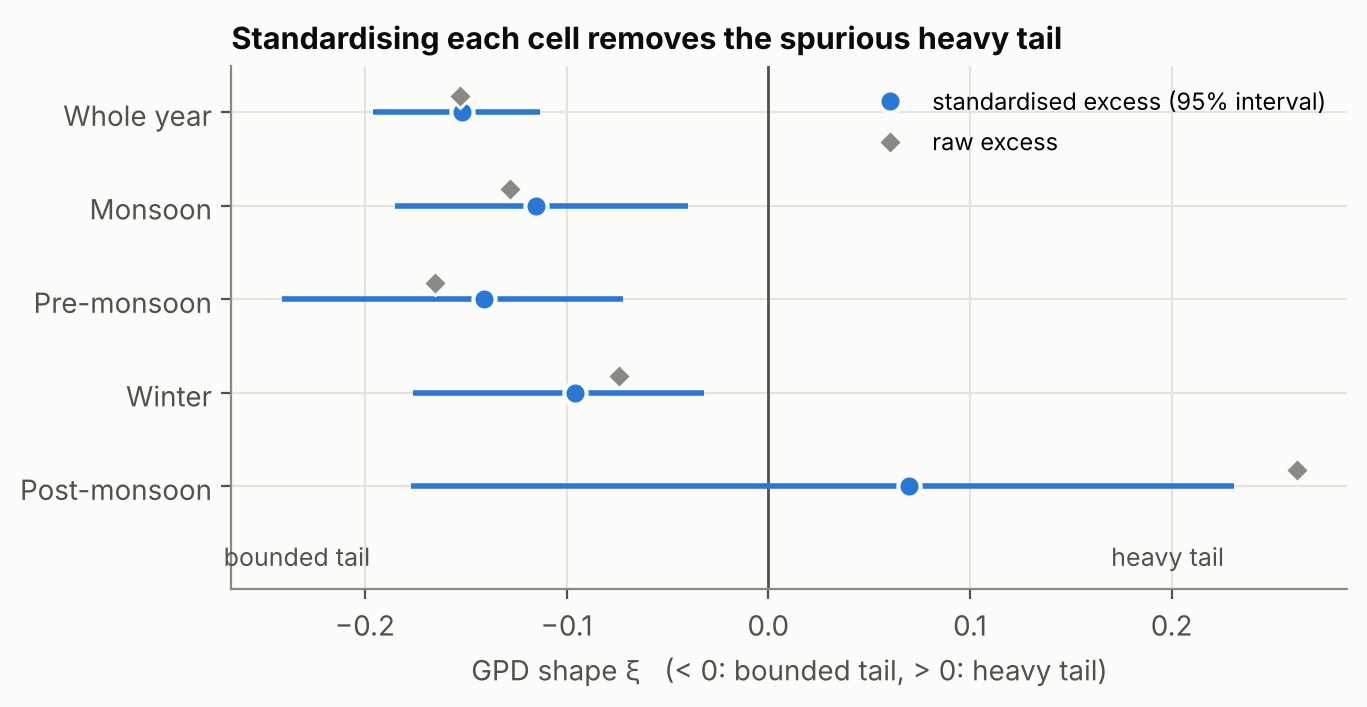
\includegraphics[width=0.75\textwidth]{fig_gpd_shape.png}
\caption{GPD shape for raw and standardised heat excesses}
\label{fig:gpdshape}
\end{figure}

Winter, pre-monsoon and monsoon have $\xi<0$: heat there has an upper limit, as expected for temperature. The
post-monsoon raw shape ($+0.26$) looked heavy-tailed partly because cells of very different variability were mixed;
standardising brings it to $+0.07$, but its interval ($-0.18$ to $+0.23$) still allows a tail without a ceiling, so
no bound is claimed for that season.

\subsection{Tail position and EVT tail focus}
The fitted GPD $F_g$ of season $g$ gives every extreme a \emph{tail position} $q=F_g(z)\in[0,1)$: $q=0.9$ means more
severe than 90\% of extreme days of that season. \textbf{EVT tail focus} draws the tail positions of the added
extremes in two equal halves: half are drawn evenly from the whole tail (0 to 1) and half evenly from its top fifth
(0.8 to 1). The share that lands in the top fifth is therefore
\begin{equation}
  0.5\times0.2+0.5\times1=0.6 ,
  \label{eq:mix}
\end{equation}
so 60\% of the added days lie in the rarest 20\% of the tail and each lower fifth receives 10\%
(Table~\ref{tab:tailmath}, Figure~\ref{fig:tailfocus}). Keeping half of the draws uniform means every part of the tail
still receives new extremes. Each $q$ is turned back into a severity $z$ by reading the fitted GPD backwards (the severity whose tail position is
$q$), and capped so that it is never above 99.9\% of the GPD's ceiling $\sigma_g/|\xi_g|$ nor above 1.5 times the
largest real severity of that season. For the post-monsoon season the fitted $\xi$ is positive, so the GPD has no
ceiling and only the second limit applies ($1.5\times1.79=2.69$).
The \emph{plain} version of each method instead uses severities as they occur in the real extremes (no EVT); a further
variant draws tail positions evenly between 0 and 1, i.e.\ the fitted GPD as it is.

\begin{table}[H]
\centering
\caption{Where the added extremes fall under EVT tail focus (per 100 added days)}
\label{tab:tailmath}
\small
\begin{tabular}{|l|c|c|c|c|c|}
\hline
\textbf{Tail position $q$} & \textbf{0--0.2} & \textbf{0.2--0.4} & \textbf{0.4--0.6} & \textbf{0.6--0.8} & \textbf{0.8--1}\\ \hline
Half drawn anywhere (50) & 10 & 10 & 10 & 10 & 10\\ \hline
Half drawn from the top (50) & 0 & 0 & 0 & 0 & 50\\ \hline
\rowcolor{rowhl}\textbf{Total (100)} & 10 & 10 & 10 & 10 & \textbf{60}\\ \hline
\end{tabular}
\end{table}

\begin{figure}[H]
\centering
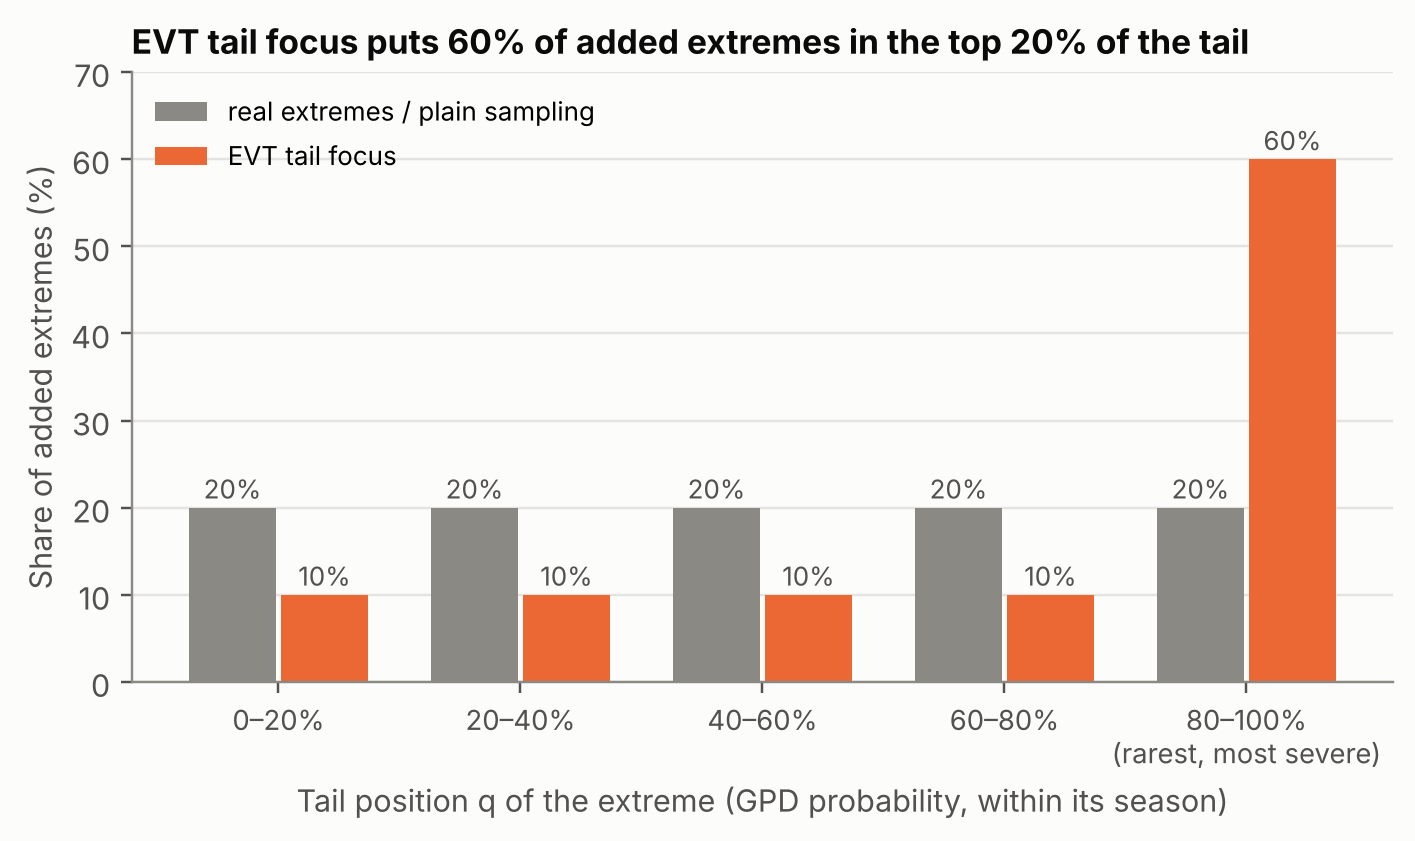
\includegraphics[width=0.75\textwidth]{fig_tail_focus.png}
\caption{Plain sampling versus EVT tail focus}
\label{fig:tailfocus}
\end{figure}

\subsection{Placement of the added extremes}
An added day is neither placed at random nor by hand. (1)~Its \emph{season} is drawn in the same proportions as the
real extremes. (2)~Its \emph{location} (latitude, longitude) is part of the generated row, learned from where real
extremes occur. (3)~The location is snapped to the nearest of the 529 cells by a nearest-neighbour search, and the row
takes that cell's real elevation and slope. (4)~The eight threshold-distance features are recomputed from that cell's
own threshold $u_{c,g}$, so the label ``extreme'' is consistent with where the day now sits. Every added row has label 1.
Like a real row, it holds the predictors of day $D$; its severity $z$ belongs to the next day $D+1$, which the row does
not contain. A synthetic row of severity $z$ therefore stands for \emph{the day before} an extreme heat day of that
severity: the diffusion model is asked for $z$ directly, and for TVAE and CTGAN the judge estimates it from the row.

\section{Generation Methods}
Each method adds one synthetic extreme per real extreme (29{,}604 rows) and is used plain and with EVT tail focus
(Table~\ref{tab:methods}). Generators that take a severity as input are asked for EVT severities directly; the others
generate a pool ten times larger, a severity ``judge'' model scores each row, and rows are selected to match the EVT
target. Every synthetic row is placed on a real grid cell and cut to valid ranges so that, for example, the minimum
temperature never exceeds the maximum. In numbers: each generator is trained on the 29{,}604 real extreme rows of the training
years (TVAE about 19 minutes, CTGAN about 24, diffusion about 30, on a free Colab T4 GPU); TVAE and CTGAN generate a
pool of 296{,}040 rows (ten per real extreme); after clean-up, 88{,}812 rows (three per real extreme) are kept per set,
at random (plain) or by EVT selection; and for each seed 29{,}604 of them are drawn and added to the
$\approx$2.9 million real training rows. The diffusion model produces 256{,}428 rows per set (8.7 per real extreme),
from which 29{,}604 are drawn in the same way for each seed.

\begin{table}[H]
\centering
\caption{Generation methods}
\label{tab:methods}
\small
\begin{tabular}{|l|l|l|}
\hline
\textbf{Family} & \textbf{Methods} & \textbf{How EVT is applied}\\ \hline
Interpolation & SMOTE, Borderline-SMOTE, ADASYN & -- \\ \hline
VAE, GAN & TVAE, CTGAN & Selection from a pool \\ \hline
Diffusion & Conditional diffusion model (built here) & Severity requested \\ \hline
Control (no generator) & Copies or weights of real extremes & Selection / weighting \\ \hline
\end{tabular}
\end{table}

\section{Generator Architectures}
\label{sec:arch}
All three generators are trained from scratch on the same 29{,}604 real extreme rows of the training years. A row has
49 base features (terrain, weather of the last three days and summaries of the last 1--4 weeks) and the season; the
eight threshold-distance features are not generated but recomputed after placement. Table~\ref{tab:arch} summarises
the three networks; TVAE and CTGAN use the standard architectures of the authors' \texttt{ctgan} library, and the
conditional diffusion model was built for this project.

\begin{table}[H]
\centering
\caption{Generator architectures and training settings}
\label{tab:arch}
\footnotesize
\begin{tabularx}{\textwidth}{|l|X|X|X|}
\hline
 & \textbf{TVAE} & \textbf{CTGAN} & \textbf{Conditional DDPM}\\ \hline
Type & Variational autoencoder & Conditional Wasserstein GAN & Denoising diffusion model\\ \hline
Input handling & Mode-specific normalisation (Gaussian mixture, $\le$10 modes); season one-hot & Same as TVAE & Quantile transform of each feature to a standard normal\\ \hline
Network & Encoder $128\!\to\!128$ (ReLU) to a 128-number code; decoder $128\!\to\!128$ (ReLU) & Generator: 2 residual layers of 256 (BatchNorm, ReLU); critic: $256\!\to\!256$ (LeakyReLU 0.2, dropout 0.5), pac 10 & Input, time and condition embeddings to 512; 4 residual blocks (LayerNorm, $512\!\to\!1024\!\to\!512$, SiLU); output 49\\ \hline
Latent / noise & 128-d code & 128-d noise + season condition & 49-d noise, 1{,}000 steps\\ \hline
Conditioning & None & Season (training-by-sampling) & Season and severity $z$, classifier-free\\ \hline
Loss & ELBO: reconstruction ($\times2$) + KL & WGAN-GP + condition cross-entropy & MSE on the added noise\\ \hline
Optimiser & Adam, weight decay $10^{-5}$ & Adam, $2\!\times\!10^{-4}$, $\beta=(0.5,0.9)$ & AdamW, $10^{-3}$, cosine decay, EMA 0.999\\ \hline
Training & 300 epochs, batch 500 & 300 epochs, batch 500 & 15{,}000 steps, batch 1{,}024\\ \hline
New sample & Random code $\to$ decoder & Noise + season $\to$ generator & 50 DDIM steps, guidance $w=2$\\ \hline
Source & Xu et al.~\cite{xu2019ctgan} & Xu et al.~\cite{xu2019ctgan} & Ho et al.~\cite{ho2020ddpm}; built here\\ \hline
\end{tabularx}
\end{table}

\subsection{TVAE}
Each continuous column is normalised \emph{per mode}: a variational Gaussian mixture splits it into up to ten modes and
a value is coded by its mode and its position within it; the season is one-hot. The encoder (two fully connected layers
of 128 units, ReLU) turns a row into a 128-number code, drawn with a little randomness around a learned centre. The
decoder (two layers of 128, ReLU) rebuilds the row from the code. Training balances two goals: rebuild each row well
(weighted by 2), and keep the codes close to a standard bell curve so that any random code decodes to a sensible row.
A new day is made by decoding a random code
(Figure~\ref{fig:arch-tvae}). Because the reconstruction rewards typical rows, its extremes are mostly mild.

\begin{figure}[H]
\centering
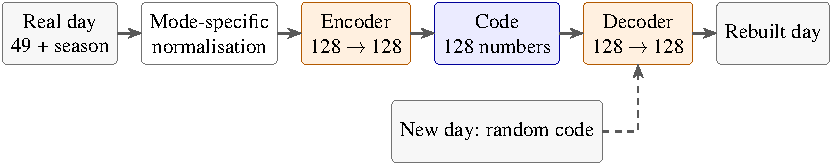
\includegraphics{diagram5.pdf}
\caption{TVAE architecture}
\label{fig:arch-tvae}
\end{figure}

\subsection{CTGAN}
The data are prepared as for TVAE. The generator takes 128-dimensional Gaussian noise concatenated with a conditional
vector (the one-hot code of a chosen season) and passes it through two residual layers of 256 units (linear,
BatchNorm, ReLU, output concatenated with the input); scalar outputs use $\tanh$ and mode and season indicators use
Gumbel-softmax. The critic sees ten rows at once (\emph{PacGAN}, pac 10) through two layers of 256 units (LeakyReLU 0.2,
dropout 0.5). Training uses the Wasserstein loss with gradient penalty (WGAN-GP)~\cite{gulrajani2017wgangp}: the critic gives each
row a realness score instead of a yes/no answer, and a penalty (weight 10) keeps that score changing smoothly, which
makes training more stable. A further term makes the generator respect the requested season. \emph{Training-by-sampling} draws
the condition so that rare seasons are seen often enough (Figure~\ref{fig:arch-ctgan}).

\begin{figure}[H]
\centering
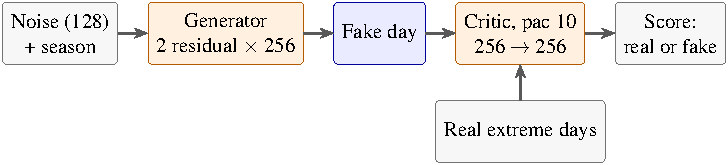
\includegraphics{diagram6.pdf}
\caption{CTGAN architecture}
\label{fig:arch-ctgan}
\end{figure}

\subsection{Conditional diffusion model}
Each of the 49 features is first mapped to a standard normal by a quantile transform. The forward process adds
Gaussian noise over 1{,}000 steps, with the amount at each step set by a cosine schedule~\cite{nichol2021improved}.
The denoising network is given the noisy row, the step number and the condition, and predicts the noise that was
added. It embeds the noisy row (linear, $49\to512$), the step number (128 sinusoidal features, then $512$, SiLU, $512$) and the
condition $c$ (season one-hot, severity $z$ and a presence flag; 6 values, then $512$, SiLU, $512$), adds the three
embeddings and applies four residual blocks (each normalises its input, widens it, applies SiLU, narrows it back and adds the input back) with widths
$512\to1024\to512$, followed by LayerNorm and a linear layer back to 49 values (Figure~\ref{fig:arch-ddpm}); it has
about 4.85 million parameters. Training minimises the squared error of the predicted noise, with the
condition dropped (set to zero) 10\% of the time, AdamW (learning rate $10^{-3}$, weight decay $10^{-4}$, cosine decay),
gradient clipping at 1, an exponential moving average of the weights (0.999), 15{,}000 steps and batches of 1{,}024.
New days are made from pure noise in 50 deterministic DDIM steps~\cite{song2021ddim} with classifier-free
guidance~\cite{ho2022cfg}: at each step the network's noise prediction with the condition is pushed away from its
prediction without it (guidance strength 2), so the new day follows the requested season and EVT severity
(Section~\ref{sec:evtmodel}) more closely; the result is mapped back by the inverse quantile
transform.

\begin{figure}[H]
\centering
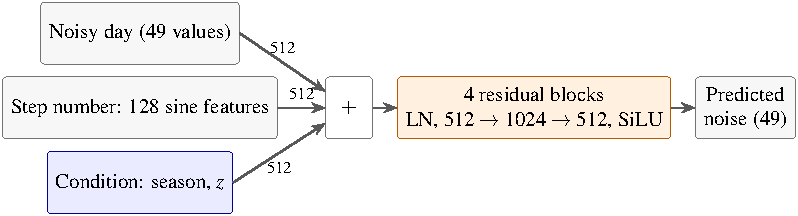
\includegraphics{diagram7.pdf}
\caption{Conditional diffusion denoiser}
\label{fig:arch-ddpm}
\end{figure}

\subsection{Severity judge for TVAE and CTGAN}
TVAE and CTGAN cannot be asked for a severity, so a LightGBM regressor (the \emph{judge}), trained on the real extremes,
predicts $z$ for each of the 296{,}040 pooled rows. Rows are grouped into 20 equal tail-position bins and drawn so that
the bins and seasons match the EVT target (60\% of the mass in the top four bins), giving 88{,}812 rows per set.

\section{Classifier and Evaluation}
\label{sec:metricsdef}
LightGBM~\cite{ke2017lightgbm} is identical for every method. Because 98\% of days are normal, accuracy is
uninformative; we report PR-AUC (average precision) on all days, on \emph{onset} days (rows where today's maximum is still below tomorrow's threshold) and on
\emph{severe} days (the 10\% most severe extremes), plus precision and recall. Table~\ref{tab:metrics} defines every
measure; Section~\ref{sec:allmetrics} compares the methods on all of them and explains why PR-AUC is the main
measure. In Table~\ref{tab:metrics}, a \emph{hit} is an extreme day that received a warning, a \emph{miss} an extreme day without one, and a
\emph{false alarm} a normal day that received one.

\begin{table}[H]
\centering
\caption{Evaluation measures (all computed on the test years 2016--2025)}
\label{tab:metrics}
\footnotesize
\begin{tabularx}{\textwidth}{|>{\raggedright\arraybackslash}p{3.0cm}|X|>{\raggedright\arraybackslash}p{2.6cm}|}
\hline
\textbf{Measure} & \textbf{Definition} & \textbf{Range}\\ \hline
Precision & hits / (hits + false alarms): share of warnings that were right & 0--1 \\ \hline
Recall & hits / (hits + misses): share of extreme days that were warned & 0--1 \\ \hline
False-alarm rate & false alarms / all normal days & 0--1 \\ \hline
CSI & hits / (hits + misses + false alarms), the critical success index of weather forecasting & 0--1 \\ \hline
PR-AUC (average precision) & Area under the precision--recall curve: the precision averaged over all warning cut-offs,
  weighted by the gain in recall & 0--1; random = share of extreme days ($\approx$0.02) \\ \hline
PR-AUC, onset days & PR-AUC computed only on rows where today's maximum temperature is still below tomorrow's threshold; the extreme days among them are the first day of a hot spell (not necessarily an IMD heat wave; it can be a single day) & as above \\ \hline
PR-AUC, severe days & PR-AUC computed on all normal days plus only the 10\% most severe extreme days (largest standardised excess $z$, taken over all test extremes pooled across seasons); the other extreme days are left out & as above \\ \hline
Warning cut-off & The probability above which a warning is given; chosen to maximise F1 on 2011--2015 & -- \\ \hline
\end{tabularx}
\end{table} Each method is trained with five seeds;
differences are tested by resampling whole test months (Section~\ref{sec:paired}). The baseline is
\emph{persistence}: ``tomorrow will be like today'', scored with today's distance to tomorrow's threshold
(\texttt{dist\_l0}) as its warning score, so that it can be ranked like a probability; this is why it has some skill on
onset days, where today is still below the threshold.

\textbf{Neural-network comparison.} A multilayer perceptron (three hidden layers of 256 units, SiLU, dropout 0.1,
sigmoid output; inputs standardised and clipped to $\pm10$; binary cross-entropy; AdamW, learning rate $10^{-3}$;
6 epochs, 2 seeds) was tried in an early run on the same inputs. On real data alone it scored about the same as LightGBM
on all days (PR-AUC 0.597 vs 0.594) and better on the most severe days (0.576 vs 0.461; the MLP was averaged over two seeds, LightGBM was a single seed in that run). However, every
synthetic data set made the MLP worse on all three scores, while LightGBM gained on the most severe days (0.461
to 0.580 with EVT-guided diffusion days); since this project tests what added extreme days do, LightGBM was kept.
It also trains on a normal CPU, and tree ensembles are generally strong on tabular data~\cite{grinsztajn2022tree}.

% =============================================================================
\chapter{Results and Discussion}
\label{ch:results}
% =============================================================================
\section{Lessons from the First Experiments}
\label{sec:lessons}
\begin{itemize}
  \item With real data alone, LightGBM was weaker than persistence on the most severe days (0.461 vs 0.565, a single
        early run).
  \item Too much synthetic data (8.7 per real extreme) hurt onset skill; one per real extreme was best.
  \item A single training run was misleading: one result reversed with other seeds, so all later results use five seeds.
  \item Drawing severities from the fitted GPD as it is gave no gain; focusing on the upper tail did.
\end{itemize}

\section{Properties of the Generators}
\begin{table}[H]
\centering
\caption{Generators before any classifier}
\label{tab:genstats}
\small
\begin{tabular}{|l|c|c|c|}
\hline
\textbf{Generator} & \makecell{\textbf{Raw rows}\\\textbf{breaking physics}} & \makecell{\textbf{Follows requested}\\\textbf{severity}$^{\dagger}$} & \makecell{\textbf{Training}\\\textbf{time}} \\ \hline
TVAE / CTGAN & 69--75\% & -- & about 19--24 min \\ \hline
Conditional diffusion & 0.0--0.2\%$^{*}$ & 0.62--0.67 (real: 0.78) & 30 min \\ \hline
\end{tabular}

\vspace{2pt}{\footnotesize $^{*}$ For the diffusion model only the temperature order was recorded: 0.0--0.2\% of rows needed reordering.\\
$^{\dagger}$ Spearman rank correlation between the requested severity and the judge's estimate of it; the value for
held-out real extremes (0.78) is the best achievable.}
\end{table}
``Raw rows breaking physics'' counts generated rows that broke at least one simple consistency rule (for example
minimum above maximum temperature, humidity outside 0--100\%, negative rain) before the clean-up. TVAE and CTGAN
broke one in most rows. Only the diffusion model could be asked for a severity and followed it closely.

\section{Comparison of Generation Methods}
\begin{figure}[H]
\centering
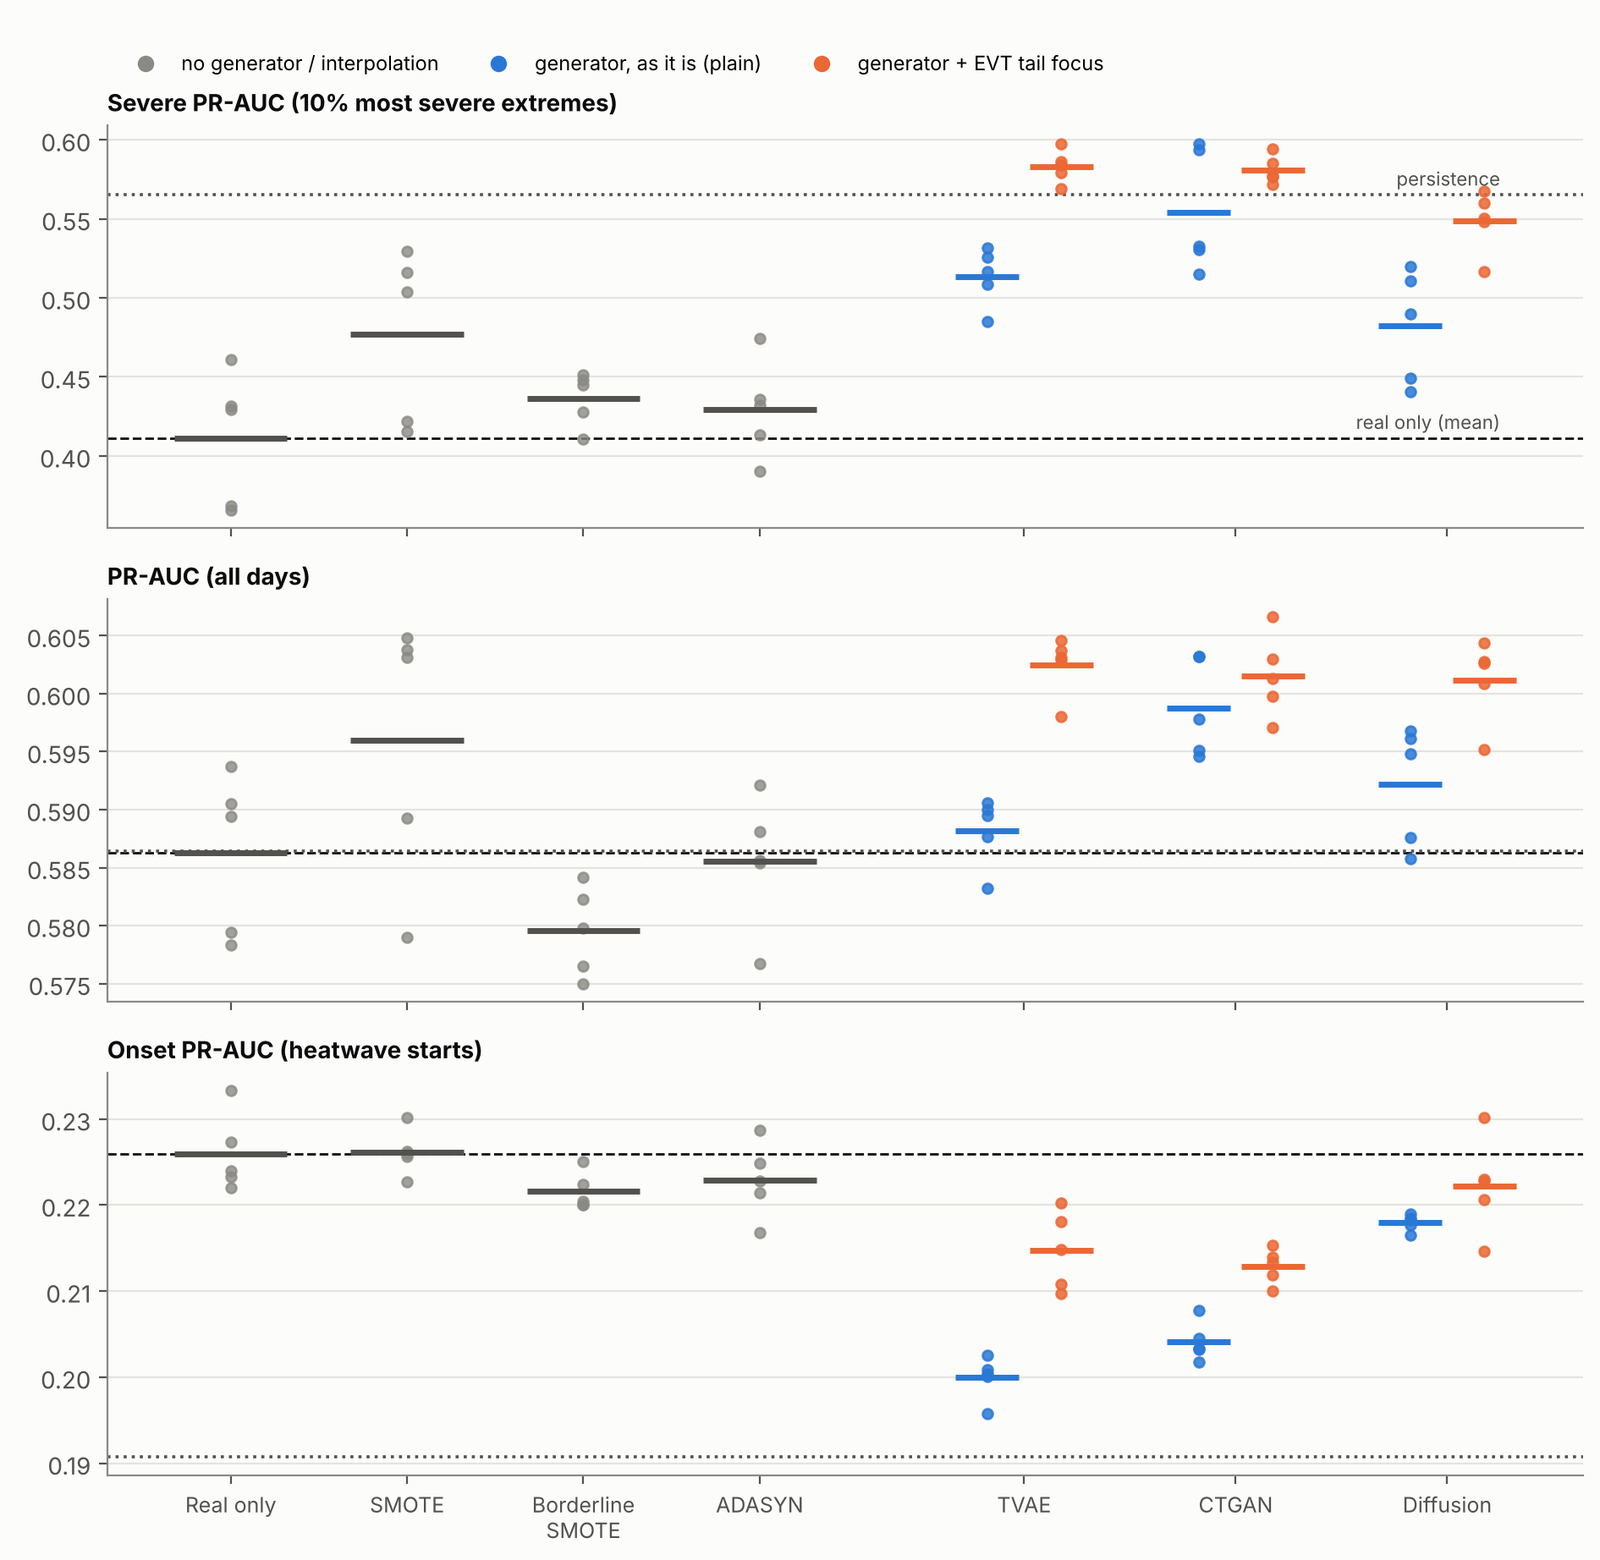
\includegraphics[width=\textwidth]{fig_step12_by_seed.png}
\caption{Test scores of every method over five training seeds (dots) and their mean (bar)}
\label{fig:step12}
\end{figure}

\begin{figure}[H]
\centering
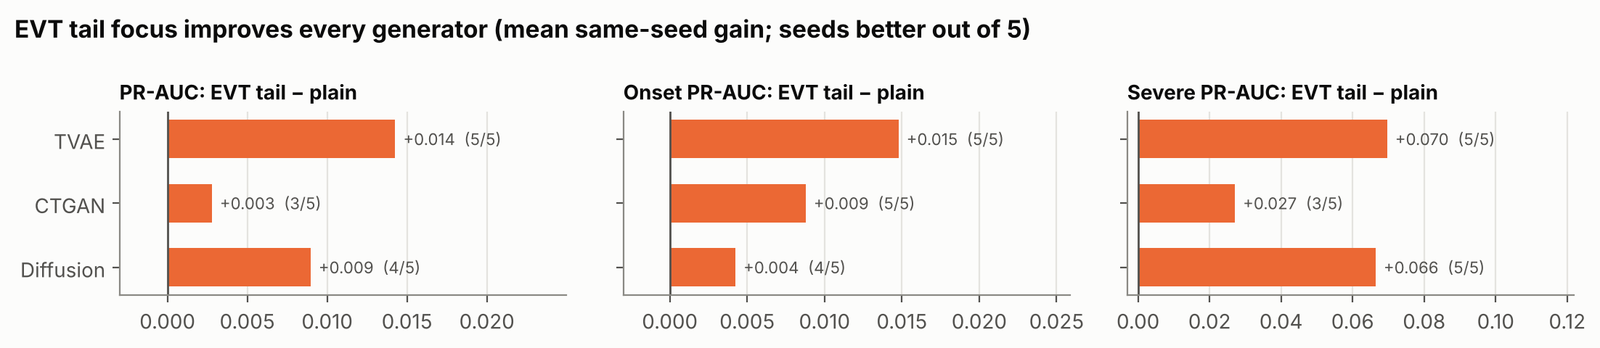
\includegraphics[width=\textwidth]{fig_evt_gain.png}
\caption{Gain of EVT tail focus over the same generator without it}
\label{fig:evtgain}
\end{figure}

\begin{table}[H]
\centering
\caption{Main results (combined prediction of five seeds, test 2016--2025, PR-AUC)}
\label{tab:rank}
\small
\begin{tabular}{|l|c|c|c|}
\hline
\textbf{Method} & \textbf{All days} & \textbf{Onset days} & \textbf{Most severe days}\\ \hline
Real data only & 0.599 & 0.235 & 0.441 \\ \hline
SMOTE & 0.604 & 0.231 & 0.507 \\ \hline
\rowcolor{rowhl} Diffusion + EVT tail & 0.609 & 0.228 & 0.579 \\
\rowcolor{rowhl} TVAE + EVT tail & 0.610 & 0.220 & \textbf{0.601} \\
\rowcolor{rowhl} CTGAN + EVT tail & 0.611 & 0.223 & \textbf{0.601} \\ \hline
\rowcolor{rowhl2} EVT-tail copies of real extremes (Section~\ref{sec:control}) & \textbf{0.613} & \textbf{0.239} & 0.530 \\ \hline
Persistence (no model) & 0.586 & 0.191 & 0.565 \\ \hline
\end{tabular}
\end{table}

\begin{itemize}
  \item \textbf{Two kinds of number.} Tables~\ref{tab:rank} and~\ref{tab:allmetrics} score the \emph{combined}
        prediction of the five seeds; Tables~\ref{tab:evtgain}, \ref{tab:ablation}, \ref{tab:other} and \ref{tab:step13}
        give the \emph{mean of five separately scored runs}, which is a little lower. For example, real data only
        scores 0.441 combined and 0.411 as a mean of runs on severe days; the 0.461 in Section~\ref{sec:lessons} is a
        single early run.
  \item \textbf{EVT tail focus improved every generator} on average on all three scores (Figure~\ref{fig:evtgain}),
        most consistently on onset days; all three top methods on validation used it.
  \item \textbf{Added data costs a little onset skill.} Every augmented method scored below real data only on onset
        days (0.220--0.231 vs 0.235; for CTGAN + EVT the loss appeared in 98\% of month resamples). Only EVT-tail
        copies of real extremes raised it (0.239). The gain is on the most severe days.
  \item \textbf{Best overall:} EVT-tail copies of real extremes have the best all-days and onset scores; CTGAN and
        TVAE with EVT tail focus have the best severe-day score.
  \item \textbf{CTGAN and TVAE with EVT tail focus were best} on the most severe days (0.601 vs 0.441 for real data
        only), and beat persistence on overall skill (0.611 vs 0.586). The top EVT-tail methods are close: CTGAN + EVT beat
        diffusion + EVT on severe days in 92\% of month resamples and TVAE + EVT in 88\%, short of the 95\% used here
        for a clear win (Section~\ref{sec:paired}).
  \item \textbf{Interpolation helps little:} SMOTE gave a small gain; Borderline-SMOTE and ADASYN none.
\end{itemize}

\textbf{Effect of EVT tail focus.} Comparing each generator with its own plain version isolates the effect
of EVT (Table~\ref{tab:evtgain}).

\begin{table}[H]
\centering
\caption{Plain versus EVT tail focus, severe-day PR-AUC (mean of five runs, each scored on its own)}
\label{tab:evtgain}
\small
\begin{tabular}{|l|c|c|c|c|c|}
\hline
\textbf{Generator} & \textbf{Plain} & \textbf{EVT tail} & \textbf{Gain} & \textbf{Runs better} & \textbf{Onset days}\\ \hline
Diffusion & 0.482 & 0.549 & +13.8\% & 5/5 & +1.9\% (4/5)\\ \hline
TVAE & 0.514 & 0.583 & +13.6\% & 5/5 & +7.4\% (5/5)\\ \hline
CTGAN & 0.554 & 0.581 & +4.9\% & 3/5 & +4.3\% (5/5)\\ \hline
\multicolumn{6}{|l|}{Real data only: 0.411 (mean of five runs).}\\ \hline
\end{tabular}
\end{table}

\textbf{Which use of EVT helps.} Because the diffusion model takes a severity, it was used to compare ways of choosing
severities with everything else fixed (Table~\ref{tab:ablation}). Sampling the fitted GPD as it is gave no gain over
real severities, since most of its mass is mild extremes; focusing on its upper 20\% did. Adding 8.7 synthetic days per
real extreme instead of one lowered onset skill (0.222 to 0.197).

\begin{table}[H]
\centering
\caption{Choice of severities for the diffusion model (severe-day PR-AUC, mean of five runs)}
\label{tab:ablation}
\small
\begin{tabular}{|l|c|c|}
\hline
\textbf{Severities requested} & \textbf{PR-AUC} & \textbf{Runs better than real severities}\\ \hline
Real data only (no synthetic days) & 0.411 & --\\ \hline
Copied from real extremes (plain) & 0.482 & --\\ \hline
Fitted GPD as it is (no tail focus) & 0.462 & 1/5\\ \hline
\rowcolor{rowhl}GPD with tail focus (Eq.~\ref{eq:mix}) & \textbf{0.549} & 5/5\\ \hline
\end{tabular}
\end{table}

\textbf{Other generators tried.} Three further generators were run in the same way: a Gaussian
copula~\cite{patki2016sdv}, CopulaGAN and a conditional WGAN-GP built in this project. EVT tail focus improved them
too (Table~\ref{tab:other}), so all six generators tried (the three main ones and these three) gained; they are left out of the main comparison for
brevity.

\begin{table}[H]
\centering
\caption{Other generators tried (severe-day PR-AUC, mean of five seeds)}
\label{tab:other}
\small
\begin{tabular}{|l|c|c|c|c|}
\hline
\textbf{Generator} & \textbf{Plain} & \textbf{EVT tail} & \textbf{Gain} & \textbf{Seeds better}\\ \hline
CopulaGAN & 0.522 & 0.578 & +10.6\% & 5/5 \\ \hline
Gaussian copula & 0.507 & 0.546 & +7.7\% & 4/5 \\ \hline
Conditional WGAN-GP & 0.509 & 0.532 & +4.5\% & 4/5 \\ \hline
\end{tabular}
\end{table}

\begin{figure}[H]
\centering
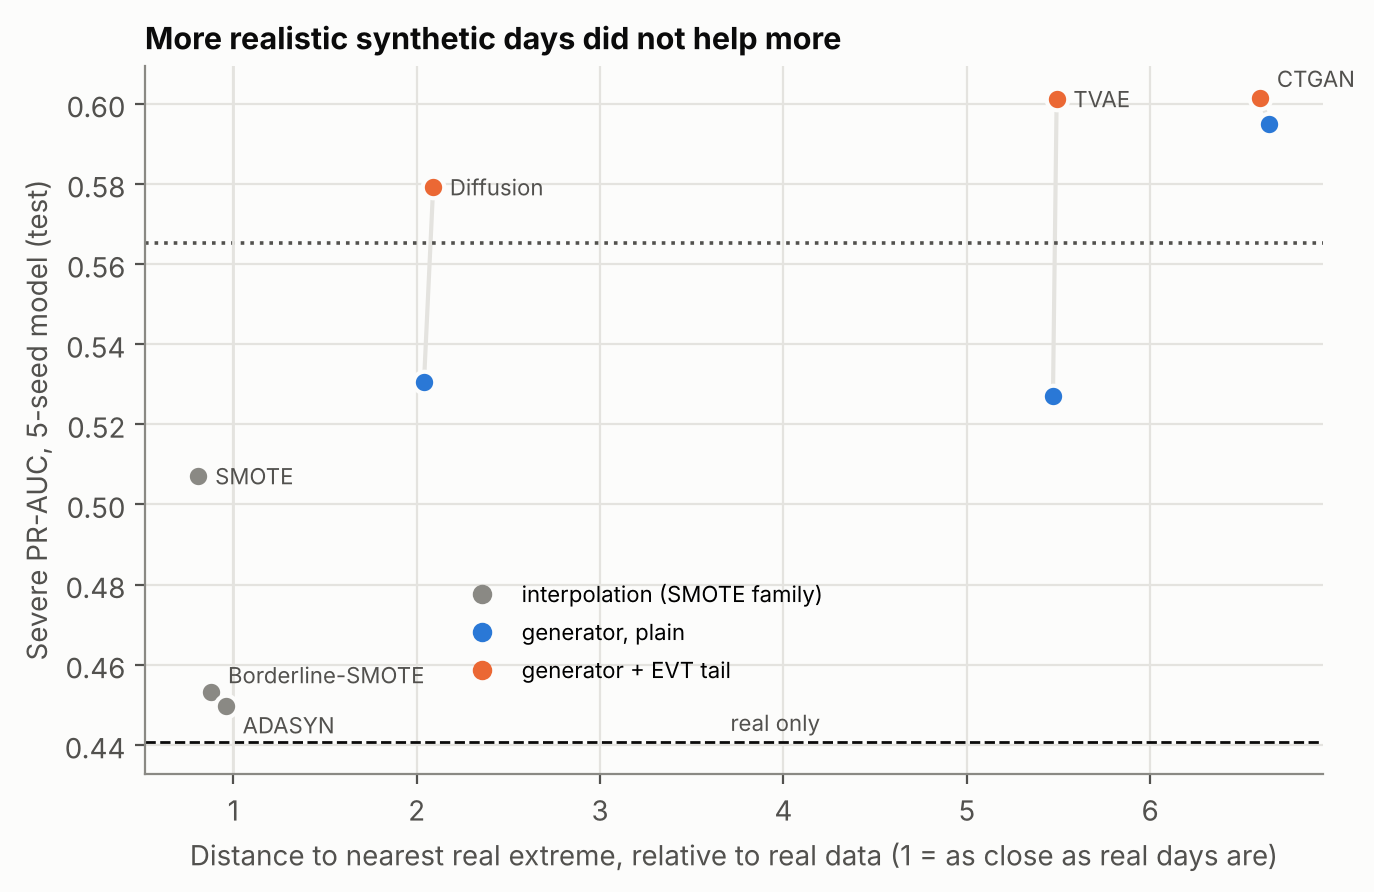
\includegraphics[width=0.78\textwidth]{fig_realism.png}
\caption{Realism of the synthetic extremes against their usefulness. Realism is the detection AUC: how well a
classifier tells synthetic extremes from real ones (0.5 = indistinguishable, 1 = always told apart).}
\label{fig:realism}
\end{figure}

\textbf{Realism is not usefulness.} Diffusion produced the most realistic days, yet CTGAN and TVAE days---easy to tell
apart from real ones---helped as much or more (Figure~\ref{fig:realism}). Where the extra days sit in the tail mattered
more than how real they looked.

\section{How Sure Are the Differences?}
\label{sec:paired}
Each comparison below resamples whole months of the test period 200 times (months are kept whole because hot days
cluster in time) and counts how often the first method beats the second. A share of at least 95\% is treated as a
clear win and at most 5\% as a clear loss.

\begin{table}[H]
\centering
\caption{Paired comparisons of the combined five-seed models: mean difference in PR-AUC and share of 200 month
resamples in which the first method is better}
\label{tab:paired}
\footnotesize
\begin{tabular}{|l|c|c|c|}
\hline
\textbf{Comparison} & \textbf{All days} & \textbf{Onset days} & \textbf{Most severe days}\\ \hline
SMOTE vs real data only & +0.004 (71\%) & $-0.004$ (22\%) & +0.055 (96\%)\\ \hline
TVAE + EVT vs real data only & +0.010 (79\%) & $-0.015$ (1\%) & +0.142 (100\%)\\ \hline
CTGAN + EVT vs real data only & +0.010 (80\%) & $-0.012$ (2\%) & +0.144 (100\%)\\ \hline
Diffusion + EVT vs real data only & +0.008 (77\%) & $-0.007$ (15\%) & +0.114 (100\%)\\ \hline
TVAE: EVT tail vs plain & +0.016 (100\%) & +0.017 (100\%) & +0.063 (96\%)\\ \hline
CTGAN: EVT tail vs plain & +0.002 (76\%) & +0.015 (100\%) & +0.004 (60\%)\\ \hline
Diffusion: EVT tail vs plain & +0.007 (97\%) & +0.004 (94\%) & +0.045 (94\%)\\ \hline
CTGAN + EVT vs persistence & +0.025 (99\%) & +0.031 (98\%) & +0.047 (92\%)\\ \hline
EVT-tail copies vs random copies & +0.005 (96\%) & +0.001 (63\%) & +0.037 (100\%)\\ \hline
CTGAN + EVT vs EVT-tail copies & $-0.003$ (34\%) & $-0.016$ (0\%) & +0.068 (93\%)\\ \hline
\end{tabular}
\end{table}

The gain on the most severe days is clear for every generator with EVT tail focus. The small changes on all days are
mostly not decisive, and the loss on onset days for the generators is clear. EVT tail focus clearly helped TVAE on
all three scores and every generator on onset days; for CTGAN on severe days it was not decisive.

% =============================================================================
\section{All Evaluation Measures and the Choice of PR-AUC}
\label{sec:allmetrics}
Table~\ref{tab:allmetrics} scores the main methods on every common measure, so that the choice of the main measure
rests on evidence. The first group of columns needs a single warning cut-off (chosen on 2011--2015, as in
Section~\ref{sec:metricsdef}); the last three columns do not. A trivial forecast that never warns is added as a
reference.

\begin{table}[H]
\centering
\caption{All evaluation measures on the test years 2016--2025 (1{,}932{,}437 rows, 37{,}450 extreme). Combined model of
five seeds. Best trained method in each column in bold. Accuracy, F1, false-alarm rate, HSS and balanced accuracy are
computed from the stored precision and recall and the known numbers of extreme and normal rows.}
\label{tab:allmetrics}
\scriptsize
\setlength{\tabcolsep}{3.2pt}
\begin{tabular}{|l|c|c|c|c|c|c|c|c||c|c|c|}
\hline
 & \multicolumn{8}{c||}{\textbf{At one warning cut-off}} & \multicolumn{3}{c|}{\textbf{All cut-offs (PR-AUC)}}\\ \hline
\textbf{Method} & \textbf{Acc.} & \textbf{Prec.} & \textbf{Recall} & \textbf{F1} & \textbf{CSI} & \textbf{FAR} & \textbf{HSS} & \textbf{Bal.\ acc.} & \textbf{All} & \textbf{Onset} & \textbf{Severe}\\ \hline
Never warn (trivial) & 98.06\% & -- & 0 & 0 & 0 & 0\% & 0 & 0.500 & 0.019 & -- & 0.002\\ \hline
Persistence (no model) & 98.29\% & 0.553 & \textbf{0.602} & 0.576 & 0.405 & 0.96\% & 0.568 & \textbf{0.796} & 0.586 & 0.191 & 0.565\\ \hline
Real data only & \textbf{98.51\%} & \textbf{0.654} & 0.495 & 0.563 & 0.392 & \textbf{0.52\%} & 0.556 & 0.745 & 0.599 & 0.235 & 0.441\\ \hline
SMOTE & 98.37\% & 0.576 & 0.594 & \textbf{0.585} & \textbf{0.413} & 0.86\% & \textbf{0.577} & 0.793 & 0.604 & 0.231 & 0.507\\ \hline
EVT-tail copies of real extremes & 98.49\% & 0.629 & 0.542 & 0.582 & 0.411 & 0.63\% & 0.575 & 0.768 & \textbf{0.613} & \textbf{0.239} & 0.530\\ \hline
Diffusion + EVT tail & 98.46\% & 0.618 & 0.541 & 0.577 & 0.405 & 0.66\% & 0.569 & 0.767 & 0.609 & 0.228 & 0.579\\ \hline
TVAE + EVT tail & 98.48\% & 0.634 & 0.511 & 0.566 & 0.394 & 0.58\% & 0.558 & 0.753 & 0.610 & 0.220 & \textbf{0.601}\\ \hline
CTGAN + EVT tail & 98.42\% & 0.600 & 0.550 & 0.574 & 0.403 & 0.72\% & 0.566 & 0.771 & 0.611 & 0.223 & \textbf{0.601}\\ \hline
\end{tabular}
\end{table}

\noindent Abbreviations: Acc.\ = accuracy; Prec.\ = precision; FAR = false-alarm rate (false alarms / normal days);
HSS = Heidke skill score (accuracy above that of chance, 0 = no skill, 1 = perfect); Bal.\ acc.\ = balanced accuracy
(mean of recall and $1-\mathrm{FAR}$). The ``--'' for onset under \emph{never warn} is because that subset's share of
extremes was not stored; for any no-skill forecast PR-AUC equals the share of extremes in the subset.

\subsection{What the table shows}
\begin{enumerate}
\item \textbf{The measures do not agree on the best method.} Accuracy, precision and false-alarm rate pick
\emph{real data only}; recall and balanced accuracy pick \emph{persistence}; F1, CSI and HSS pick \emph{SMOTE}; PR-AUC
picks EVT-tail copies (all days and onsets) and TVAE/CTGAN + EVT tail (severe days). A single main measure therefore has
to be chosen for a stated reason, before looking at the results.
\item \textbf{Accuracy cannot separate the methods.} Never warning already scores 98.06\%. All trained methods lie
between 98.37\% and 98.51\%, and the highest value goes to the most cautious model, the one that misses half of the
extreme days.
\item \textbf{Precision, recall and false-alarm rate trade against each other.} Real data only has the best precision
(0.654) and the fewest false alarms (0.52\%) because it warns least, and so it has the lowest recall (0.495).
Persistence is the reverse. Moving the cut-off moves a method along this trade-off, so one of these numbers alone says
little about how good the model is.
\item \textbf{F1, CSI and HSS depend on one cut-off chosen in other years.} The cut-off is fixed on 2011--2015, when
1.00\% of rows were extreme; in 2016--2025 the share is 1.94\%. All trained methods lie within 0.02 of each other
(F1 0.563--0.585, CSI 0.392--0.413). These
measures are reported, but a method should not be judged on them alone.
\item \textbf{Balanced accuracy and ROC-type measures are flattered by the many normal days.} Their false-alarm term
divides by 1.89 million normal days, so the false-alarm rate is below 1\% for every method. Doubling the false alarms
(0.52\% for real data only to 0.96\% for persistence) moves a model by less than 0.005 along the horizontal axis of a
ROC curve, while precision falls from 0.654 to 0.553. Persistence, which has no model, has the best balanced
accuracy.
\item \textbf{Only PR-AUC on severe days shows the purpose of the project.} The most severe extremes are 10\% of all
extreme days, so they barely move all-day measures. On them, PR-AUC rises from 0.441 (real data only) to 0.601
(TVAE/CTGAN + EVT tail), the largest difference of any measure in the table, while all-days PR-AUC does not fall
(0.599 to 0.611).
\end{enumerate}

\subsection{Why PR-AUC was chosen}
\begin{table}[H]
\centering
\caption{What each measure rewards, its problem in this task, and how it is used in this report}
\label{tab:metricchoice}
\footnotesize
\begin{tabularx}{\textwidth}{|>{\raggedright\arraybackslash}p{2.5cm}|>{\raggedright\arraybackslash}X|>{\raggedright\arraybackslash}p{4.4cm}|>{\raggedright\arraybackslash}p{2.3cm}|}
\hline
\textbf{Measure} & \textbf{Problem in this task (evidence in Table~\ref{tab:allmetrics})} & \textbf{What it is still good for} & \textbf{Use here}\\ \hline
Accuracy & Dominated by the 98\% normal days; never warning scores 98.06\% & Nothing for rare events & Not used\\ \hline
Precision / recall / FAR alone & Each can be made high by moving the cut-off; they rank methods in opposite orders & Explaining a chosen operating point to users & Reported at the chosen cut-off\\ \hline
F1, CSI, HSS & Depend on one cut-off fixed in cooler years; trained methods differ by $\le 0.02$ & Standard skill scores of weather services & Reported as supporting evidence\\ \hline
Balanced accuracy, ROC-AUC & Count correct quiet days; false alarms look tiny next to 1.89 million normal days; persistence looks best & Problems where both classes are equally important & Not used\\ \hline
\textbf{PR-AUC} (all, onset, severe) & Needs a fixed subset definition to compare (done before the experiments) & Threshold-free; looks only at how well extremes are ranked above normal days; random level equals the share of extremes, so it shows real skill & \textbf{Main measure}\\ \hline
\end{tabularx}
\end{table}

\begin{enumerate}
\item \textbf{It does not depend on a cut-off.} It averages precision over every possible warning level, so a method
is not rewarded or punished for where one cut-off happened to fall.
\item \textbf{It ignores correct quiet days.} Precision and recall contain no true-negative term, so the 1.89 million
normal days cannot hide errors on the 37{,}450 extreme ones.
\item \textbf{Its no-skill level is known and low.} A random forecast scores the share of extremes (0.019 on all
days, 0.002 on severe days), so 0.60 is clearly far above chance.
\item \textbf{It can be computed on any subset.} The same measure on onset and severe days answers the two questions of
the project: can the model see heat coming, and can it rank the worst days first.
\item \textbf{It is the recommended measure for rare events.} Saito and Rehmsmeier~\cite{saito2015pr} showed that PR
curves describe performance on imbalanced data more faithfully than ROC curves, and Davis and
Goadrich~\cite{davis2006pr} showed that a method can dominate in ROC space without being better in PR space.
\end{enumerate}

\section{Control Experiment: Is a Generator Needed?}
\label{sec:control}
\begin{figure}[H]
\centering
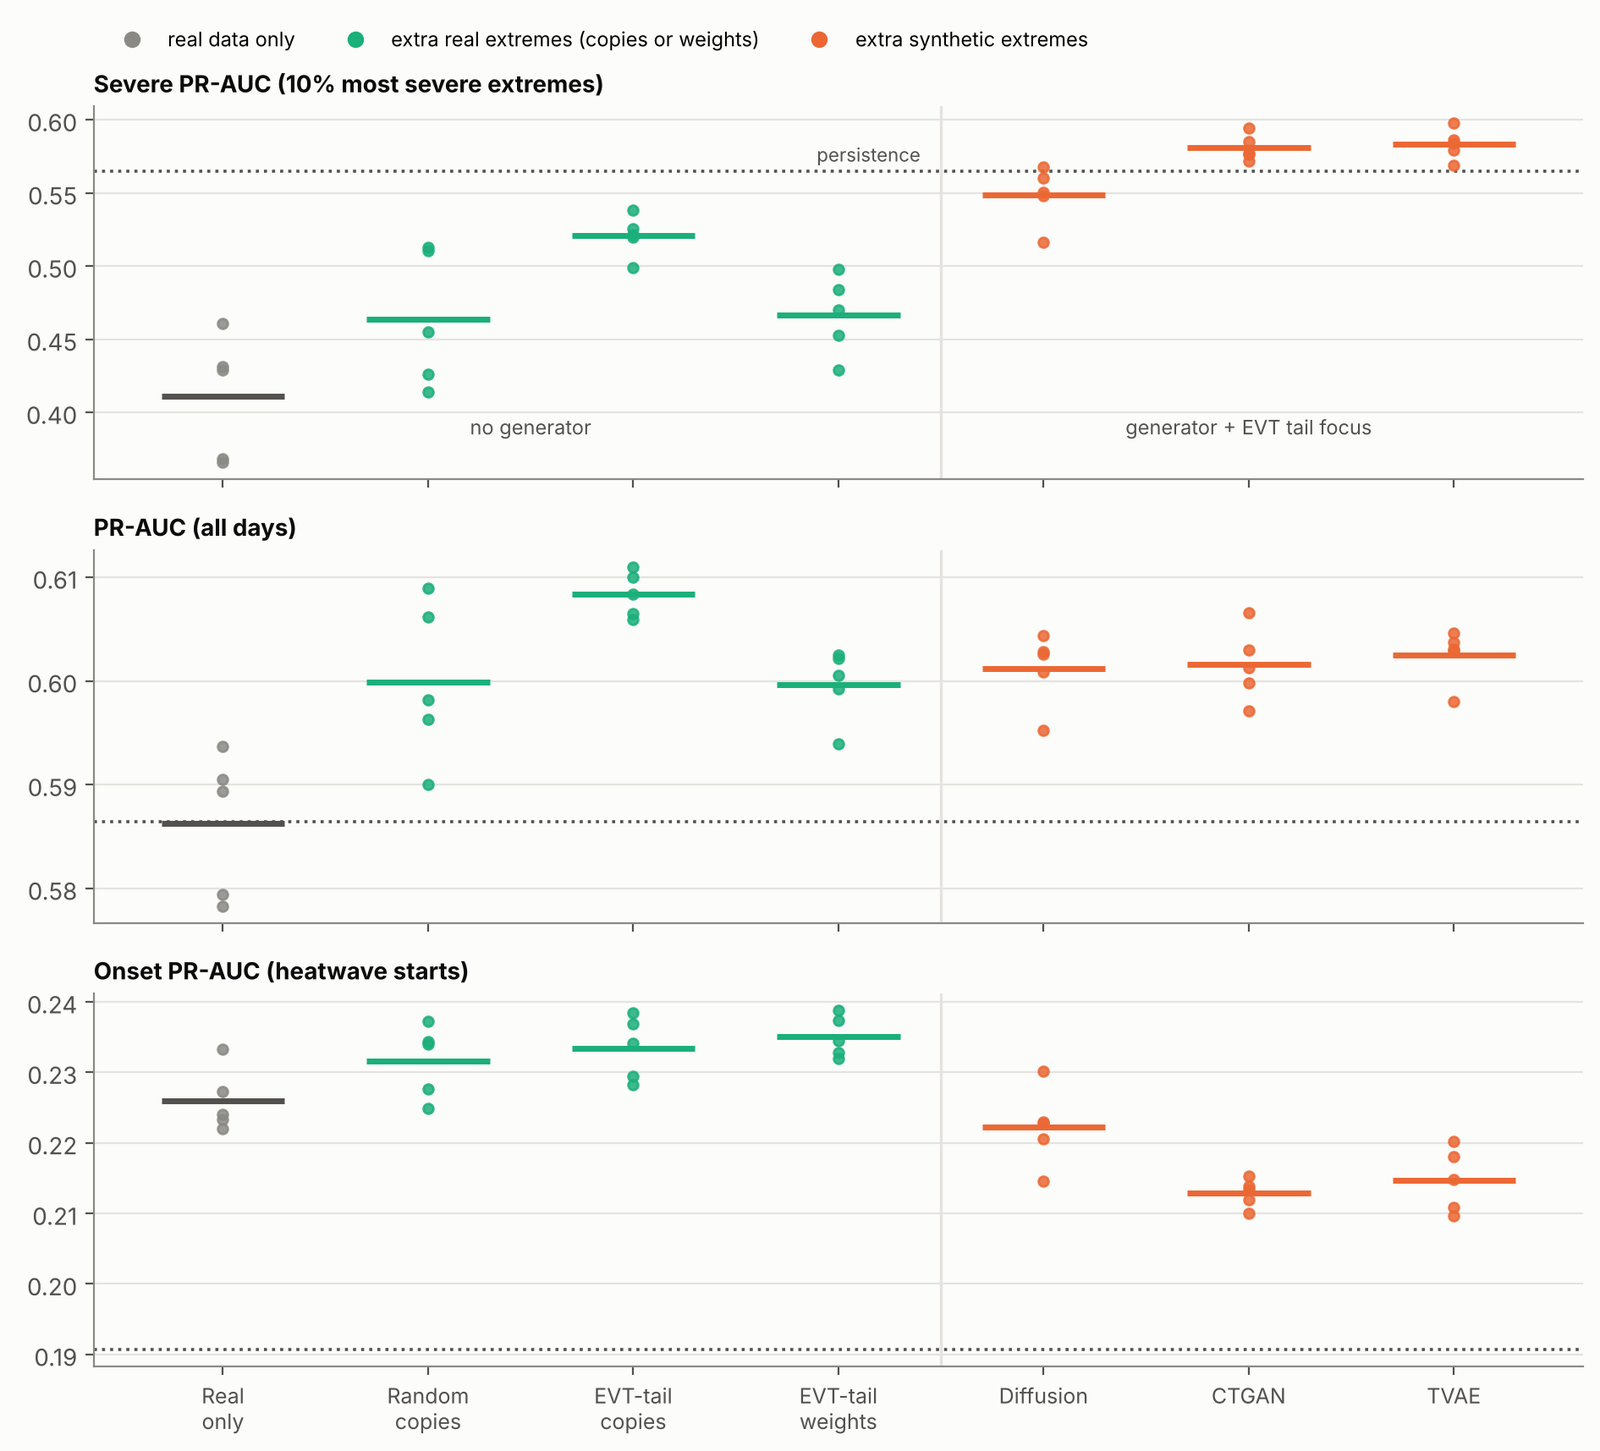
\includegraphics[width=0.85\textwidth]{fig_step13.png}
\caption{EVT tail emphasis with and without a generator}
\label{fig:step13}
\end{figure}

\begin{table}[H]
\centering
\caption{Control experiment (mean of five seeds, PR-AUC)}
\label{tab:step13}
\small
\begin{tabular}{|l|c|c|c|}
\hline
\textbf{Method} & \textbf{All days} & \textbf{Onset days} & \textbf{Most severe days}\\ \hline
Random copies of real extremes & 0.600 & 0.232 & 0.464 \\ \hline
\rowcolor{rowhl2} EVT-tail copies of real extremes & \textbf{0.608} & \textbf{0.233} & 0.521 \\ \hline
CTGAN / TVAE + EVT tail & 0.602--0.603 & 0.213--0.215 & \textbf{0.581--0.583} \\ \hline
\end{tabular}
\end{table}

EVT works on its own: EVT-tail copies beat random copies on severe days in all five seeds (+0.057) and gave the best
overall score of the study. Generators add the far tail (+0.06 on severe days, 5/5 seeds) at a small cost on onset
days ($-0.02$, 5/5 seeds; CTGAN + EVT beat the EVT-tail copies on severe days in 93\% of month resamples and lost
on onset days in all of them), because copies cannot go beyond the hottest real day.

\section{What the Results Mean in Practice}
For the best model, about \textbf{6 in 10 warnings are correct} (random guessing: 2 in 100), it catches \textbf{55\%}
of extreme days a day ahead, and it raises a false alarm on about \textbf{0.7\%} of normal days. It needs only data up
to today.

\section{Limitations}
\label{sec:limits}
Results are based on reanalysis data, not yet checked against station records; only next-day heat was modelled; the
gain over persistence on all days is modest; the tail-focus setting was fixed by hand; and free compute limited
training to half of 1981--2010. The clean-up of synthetic days only cuts values to valid ranges and orders the three
daily temperatures: humidity is not recomputed after the dewpoint is capped, temperatures are not checked against
the height of the cell a row is placed on, and the 7--30-day history columns are not recomputed from the daily
values. One early design choice used test scores: the day-of-year predictors were dropped after an early run in which
they lowered the test score (on validation they had helped), so that choice was not made on validation alone. Two of
the 57 columns (\texttt{dist\_trend} and \texttt{tmax\_change}) are identical, so the model has 56 distinct
predictors; for a tree model a duplicate column changes little.

% =============================================================================
\chapter{Conclusion and Future Work}
% =============================================================================
\section{Conclusions}
\begin{enumerate}
  \item Modelling heat extremes as a tail with a GPD gives bounded tails in winter, pre-monsoon and monsoon (the
        post-monsoon tail is not clearly bounded), and the fixed thresholds show a doubling of heat extremes in
        2016--2025.
  \item Using EVT to focus added extremes on the rarest part of the tail improved every generator, and works even with
        simple copies of real days, which gave the best all-days and onset scores.
  \item CTGAN and TVAE with EVT tail focus gave the best results on the most severe days and beat persistence overall,
        at a small cost on onset days.
  \item Where synthetic extremes are placed matters more than how realistic they are.
\end{enumerate}

\section{Future Work}
Validate severe days against weather stations; tune the tail focus; build EVT into generator training; predict
several days ahead with neighbouring cells; and test the framework on other imbalanced data sets.

% =============================================================================
%  TIMELINE / OUTCOMES
% =============================================================================
\clearpage
\leftchapter{Timeline/ Outcomes}
% Edit the weeks below to match your actual schedule: \gA / \gB = filled cell, empty = nothing.
\newcommand{\gB}{\cellcolor{ganttB}}
\newcommand{\gA}{\cellcolor{ganttA}}
\begin{table}[H]
\centering
\small
\setlength{\tabcolsep}{4pt}
\begin{tabular}{|p{5.6cm}|*{8}{p{0.62cm}|}}
\hline
\rowcolor{gray!55}
\textcolor{white}{\textbf{Outcomes}} & \multicolumn{4}{c|}{\textcolor{white}{\textbf{October 2026}}} & \multicolumn{4}{c|}{\textcolor{white}{\textbf{November 2026}}}\\ \hline
 & \centering W1 & \centering W2 & \centering W3 & \centering W4 & \centering W1 & \centering W2 & \centering W3 & \centering\arraybackslash W4 \\ \hline
Data collection and verification & \gA & \gA & & & & & & \\ \hline
Literature review & & \gA & \gA & & & & & \\ \hline
Labels, features, EVT analysis & & & \gA & \gA & & & & \\ \hline
Baselines and GAN experiments & & & & \gA & & & & \\ \hline
Diffusion model and 5-seed evaluation & & & & \gA & \gB & & & \\ \hline
Generator comparison (fixed LightGBM) & & & & & & \gB & & \\ \hline
Control experiment & & & & & & \gB & & \\ \hline
Report and presentation & & & & & \gB & & \gB & \gB \\ \hline
\end{tabular}
\caption{Project timeline}
\label{tab:timeline}
\end{table}

\textbf{Outcomes:} a verified 45-year data set of seasonal heat extremes for 529 grid cells; an extreme value model of
the heat tail; an EVT-guided conditional diffusion model; a fair comparison of six data
generation methods under a fixed classifier; and open, reproducible code that runs on free cloud resources:\\
\url{https://github.com/Divyansh-jain2/Major_Technical_Project}

% =============================================================================
%  REFERENCES
% =============================================================================
\renewcommand{\bibname}{References:}
{\titleformat{name=\chapter,numberless}[block]{\normalfont\bfseries\fontsize{22}{26}\selectfont\filright}{}{0pt}{}
\begin{thebibliography}{99}
\addcontentsline{toc}{chapter}{References}
\setlength{\itemsep}{2pt}
\small
\bibitem{coles2001} S. Coles, \reflink{https://doi.org/10.1007/978-1-4471-3675-0}{An Introduction to Statistical Modeling of Extreme Values}, Springer, 2001.
\bibitem{pickands1975} J. Pickands, \reflink{https://doi.org/10.1214/aos/1176343003}{Statistical inference using extreme order statistics}, Annals of Statistics 3 (1975) 119--131.
\bibitem{balkema1974} A. A. Balkema and L. de Haan, \reflink{https://doi.org/10.1214/aop/1176996548}{Residual life time at great age}, Annals of Probability 2 (1974) 792--804.
\bibitem{chawla2002smote} N. V. Chawla, K. W. Bowyer, L. O. Hall and W. P. Kegelmeyer, \reflink{https://doi.org/10.1613/jair.953}{SMOTE: Synthetic minority over-sampling technique}, Journal of Artificial Intelligence Research 16 (2002) 321--357.
\bibitem{han2005borderline} H. Han, W.-Y. Wang and B.-H. Mao, \reflink{https://doi.org/10.1007/11538059_91}{Borderline-SMOTE: A new over-sampling method in imbalanced data sets learning}, International Conference on Intelligent Computing, 2005.
\bibitem{he2008adasyn} H. He, Y. Bai, E. A. Garcia and S. Li, \reflink{https://doi.org/10.1109/IJCNN.2008.4633969}{ADASYN: Adaptive synthetic sampling approach for imbalanced learning}, IEEE International Joint Conference on Neural Networks, 2008.
\bibitem{elor2022smote} Y. Elor and H. Averbuch-Elor, \reflink{https://arxiv.org/abs/2201.08528}{To SMOTE, or not to SMOTE?}, arXiv:2201.08528, 2022.
\bibitem{goodfellow2014gan} I. Goodfellow et al., \reflink{https://arxiv.org/abs/1406.2661}{Generative adversarial nets}, Advances in Neural Information Processing Systems, 2014.
\bibitem{xu2019ctgan} L. Xu, M. Skoularidou, A. Cuesta-Infante and K. Veeramachaneni, \reflink{https://arxiv.org/abs/1907.00503}{Modeling tabular data using conditional GAN}, Advances in Neural Information Processing Systems, 2019.
\bibitem{kingma2014vae} D. P. Kingma and M. Welling, \reflink{https://arxiv.org/abs/1312.6114}{Auto-encoding variational Bayes}, International Conference on Learning Representations, 2014.
\bibitem{patki2016sdv} N. Patki, R. Wedge and K. Veeramachaneni, \reflink{https://doi.org/10.1109/DSAA.2016.49}{The Synthetic Data Vault}, IEEE International Conference on Data Science and Advanced Analytics, 2016.
\bibitem{ho2020ddpm} J. Ho, A. Jain and P. Abbeel, \reflink{https://arxiv.org/abs/2006.11239}{Denoising diffusion probabilistic models}, Advances in Neural Information Processing Systems, 2020.
\bibitem{gulrajani2017wgangp} I. Gulrajani, F. Ahmed, M. Arjovsky, V. Dumoulin and A. Courville, \reflink{https://arxiv.org/abs/1704.00028}{Improved training of Wasserstein GANs}, Advances in Neural Information Processing Systems, 2017.
\bibitem{nichol2021improved} A. Q. Nichol and P. Dhariwal, \reflink{https://arxiv.org/abs/2102.09672}{Improved denoising diffusion probabilistic models}, International Conference on Machine Learning, 2021.
\bibitem{song2021ddim} J. Song, C. Meng and S. Ermon, \reflink{https://arxiv.org/abs/2010.02502}{Denoising diffusion implicit models}, International Conference on Learning Representations, 2021.
\bibitem{ho2022cfg} J. Ho and T. Salimans, \reflink{https://arxiv.org/abs/2207.12598}{Classifier-free diffusion guidance}, NeurIPS Workshop on Deep Generative Models and Downstream Applications, 2021.
\bibitem{grinsztajn2022tree} L. Grinsztajn, E. Oyallon and G. Varoquaux, \reflink{https://arxiv.org/abs/2207.08815}{Why do tree-based models still outperform deep learning on typical tabular data?}, Advances in Neural Information Processing Systems (Datasets and Benchmarks), 2022.
\bibitem{kotelnikov2023tabddpm} A. Kotelnikov, D. Baranchuk, I. Rubachev and A. Babenko, \reflink{https://arxiv.org/abs/2209.15421}{TabDDPM: Modelling tabular data with diffusion models}, International Conference on Machine Learning, 2023.
\bibitem{dsouza2025overlap} A. D'souza, Swetha M and S. Sarawagi, \reflink{https://arxiv.org/abs/2412.15657}{Synthetic tabular data generation for imbalanced classification: The surprising effectiveness of an overlap class}, AAAI Conference on Artificial Intelligence, 2025.
\bibitem{bhatia2021exgan} S. Bhatia, A. Jain and B. Hooi, \reflink{https://arxiv.org/abs/2009.08454}{ExGAN: Adversarial generation of extreme samples}, AAAI Conference on Artificial Intelligence, 2021.
\bibitem{boulaguiem2022evtgan} Y. Boulaguiem, J. Zscheischler, E. Vignotto, K. van der Wiel and S. Engelke, \reflink{https://arxiv.org/abs/2111.00267}{Modeling and simulating spatial extremes by combining extreme value theory with generative adversarial networks}, Environmental Data Science 1 (2022) e5.
\bibitem{pandey2025heavy} K. Pandey et al., \reflink{https://arxiv.org/abs/2410.14171}{Heavy-tailed diffusion models}, International Conference on Learning Representations, 2025.
\bibitem{lopezgomez2023heat} I. Lopez-Gomez, A. McGovern, S. Agrawal and J. Hickey, \reflink{https://arxiv.org/abs/2205.10972}{Global extreme heat forecasting using neural weather models}, Artificial Intelligence for the Earth Systems, 2023.
\bibitem{zhang2025records} Z. Zhang, E. Fischer, J. Zscheischler and S. Engelke, \reflink{https://arxiv.org/abs/2508.15724}{Numerical models outperform AI weather forecasts of record-breaking extremes}, arXiv:2508.15724, 2025.
\bibitem{bhan_imd} S. C. Bhan, \reflink{https://heathealth.info/wp-content/uploads/Poster_SC-Bhan_FGFHH-Subhash-Bhan.pdf}{Heat wave forecasting and early warning services of the India Meteorological Department} (poster), Global Heat Health Information Network, accessed November 2026.
\bibitem{ke2017lightgbm} G. Ke et al., \reflink{https://papers.nips.cc/paper/6907-lightgbm-a-highly-efficient-gradient-boosting-decision-tree}{LightGBM: A highly efficient gradient boosting decision tree}, Advances in Neural Information Processing Systems, 2017.
\bibitem{munoz2021era5land} J. Mu\~noz-Sabater et al., \reflink{https://doi.org/10.5194/essd-13-4349-2021}{ERA5-Land: A state-of-the-art global reanalysis dataset for land applications}, Earth System Science Data 13 (2021) 4349--4383.
\bibitem{farr2007srtm} T. G. Farr et al., \reflink{https://doi.org/10.1029/2005RG000183}{The Shuttle Radar Topography Mission}, Reviews of Geophysics 45 (2007) RG2004.
\bibitem{hersbach2020era5} H. Hersbach et al., \reflink{https://doi.org/10.1002/qj.3803}{The ERA5 global reanalysis}, Quarterly Journal of the Royal Meteorological Society 146 (2020) 1999--2049.
\bibitem{srivastava2009imd} A. K. Srivastava, M. Rajeevan and S. R. Kshirsagar, \reflink{https://doi.org/10.1002/asl.232}{Development of a high resolution daily gridded temperature data set (1969--2005) for the Indian region}, Atmospheric Science Letters 10 (2009) 249--254.
\bibitem{rani2021imdaa} S. I. Rani et al., \reflink{https://doi.org/10.1175/JCLI-D-20-0412.1}{IMDAA: High-resolution satellite-era reanalysis for the Indian monsoon region}, Journal of Climate 34 (2021) 5109--5133.
\bibitem{gelaro2017merra2} R. Gelaro et al., \reflink{https://doi.org/10.1175/JCLI-D-16-0758.1}{The Modern-Era Retrospective Analysis for Research and Applications, Version 2 (MERRA-2)}, Journal of Climate 30 (2017) 5419--5454.
\bibitem{gsod} NOAA National Centers for Environmental Information, \reflink{https://www.ncei.noaa.gov/access/metadata/landing-page/bin/iso?id=gov.noaa.ncdc:C00516}{Global Surface Summary of the Day (GSOD)}, accessed November 2026.
\bibitem{eyring2016cmip6} V. Eyring et al., \reflink{https://doi.org/10.5194/gmd-9-1937-2016}{Overview of the Coupled Model Intercomparison Project Phase 6 (CMIP6) experimental design and organization}, Geoscientific Model Development 9 (2016) 1937--1958.
\bibitem{imd2022normal} India Meteorological Department, \reflink{https://internal.imd.gov.in/press_release/20220414_pr_1572.pdf}{Updated rainfall normal based on data of 1971--2020} (press release), New Delhi, 14 April 2022.
\bibitem{imd2026monsoon} India Meteorological Department, \reflink{https://mausam.imd.gov.in/Forecast/marquee_data/Salient_Features_SW_MONSOON\%20_2026_30_sep.pdf}{Salient features of the 2026 southwest monsoon season}, 30 September 2026.
\bibitem{imdheatdef} India Meteorological Department, \reflink{https://mausam.imd.gov.in/pdfs/heatcolduser/Definition.pdf}{Heat wave and warm night: definitions and criteria}, accessed November 2026.
\bibitem{naturalearth} Natural Earth, \reflink{https://www.naturalearthdata.com}{Free vector map data at 1:10m scale} (admin-0, India point of view; admin-1 states), accessed November 2026.
\bibitem{saito2015pr} T. Saito and M. Rehmsmeier, \reflink{https://doi.org/10.1371/journal.pone.0118432}{The precision-recall plot is more informative than the ROC plot when evaluating binary classifiers on imbalanced datasets}, PLOS ONE 10(3): e0118432, 2015.
\bibitem{davis2006pr} J. Davis and M. Goadrich, \reflink{https://doi.org/10.1145/1143844.1143874}{The relationship between precision-recall and ROC curves}, Proceedings of the 23rd International Conference on Machine Learning (ICML), 2006.
\bibitem{funk2015chirps} C. Funk et al., \reflink{https://doi.org/10.1038/sdata.2015.66}{The climate hazards infrared precipitation with stations: a new environmental record for monitoring extremes}, Scientific Data 2, 150066, 2015.
\end{thebibliography}}

\end{document}